\chapter{仰角データ取得システムの改善}

CMB観測においては、検出器の時系列データと望遠鏡の角度データを途切れることなく連続的に取得し続けなければいけない。そのため、角度データ取得システムは安定的でかつ操作性がよいものであることが求められる。本章では既存の望遠鏡の仰角データ取得システムを改善し、その動作確認を行なった。
\section{望遠鏡仰角データ取得システムの改善}

\subsection{角度情報データ取得の概要}
はじめに、GroundBIRD全体でのデータ取得システムの概要を述べる。CMB観測においては検出器の信号を時系列データ(以下、TODと略す)として取得する。最終的なマップ作成のためには、TODと同期して望遠鏡の視線情報(角度データ)を取得することが求められる。GroundBIRDでは望遠鏡の仰角方向と方位角方向で2つの角度データを取得している。連続回転する回転台の上部と下部は回転継手によって電気的に接続されている(図\ref{GB_daq})。

\begin{figure}[htbp]
  \centering
  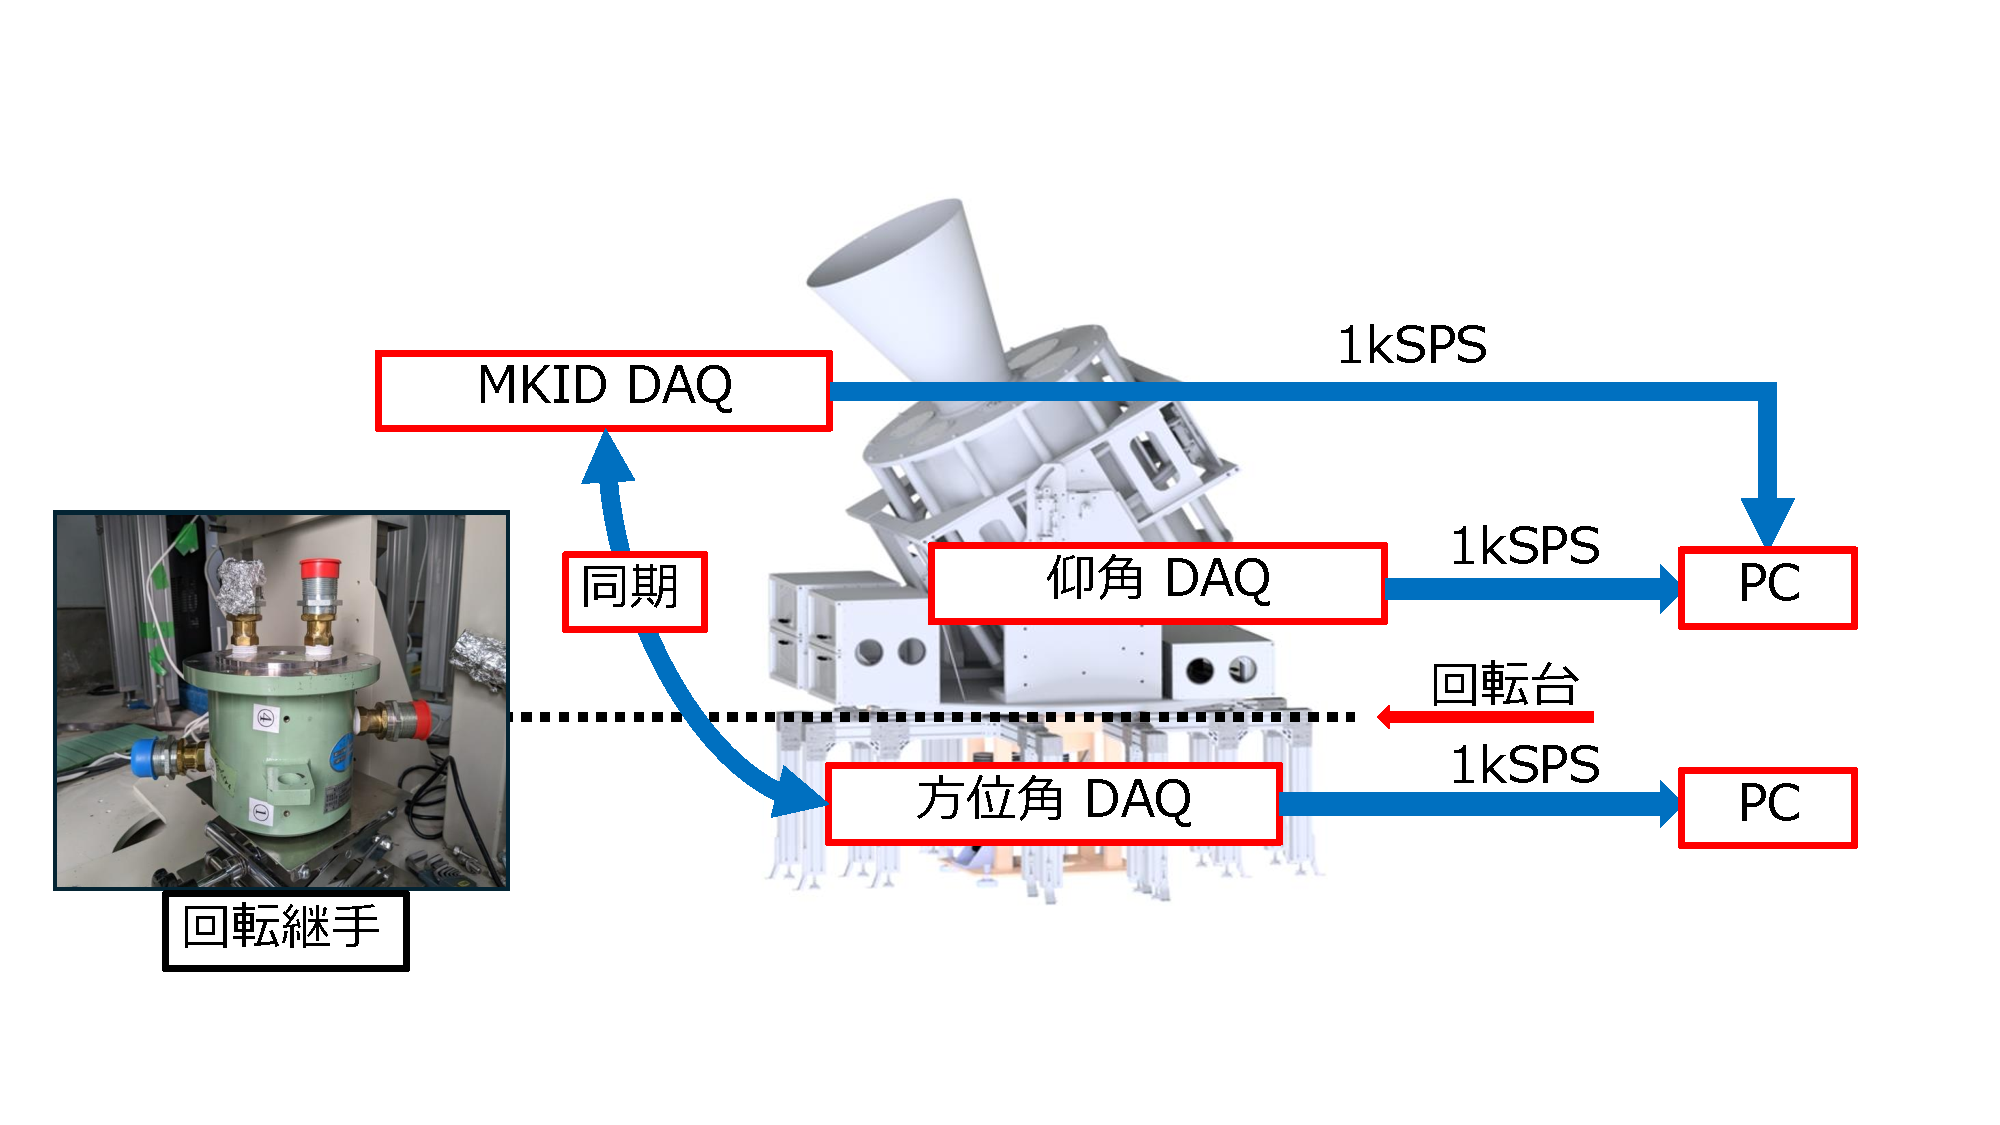
\includegraphics[width=1.0\columnwidth]{4_elDAQ/figs/GB_daq_2.pdf}
  \caption{GroundBIRDの検出器データと角度データ取得系の概要。回転する回転台の上下での信号同期は``回転継手''が担っている。}
  \label{GB_daq}
\end{figure}

仰角方向の角度データは、望遠鏡の側面に取り付けられたロータリーエンコーダー(Canon, R-1SL \cite{R-1SL})を使用し、Digilent製のFPGAボードZybo Z7-20 (\cite{Zybo}、以下では単にZyboと記す)で読み出す(図\ref{el_daq})。FPGAとはField Programmable Gate Array の略で、様々な論理回路がチップに搭載されており、使用者が配線を自由に組み合わせて論理回路を作ることができるデバイスである。FPGAでは特定の演算を行う回路を作成できるため、高速処理を可能にする。また並列処理も得意である。エンコーダーは4秒角($1.1\cdot {10^{-3}}^{\circ}$)もの高い角度分解能を持つ。

\begin{figure}[h]
  \begin{tabular}{cc}
    %---- 最初の図 ---------------------------
    \begin{minipage}[t]{0.45\hsize}
      \centering
      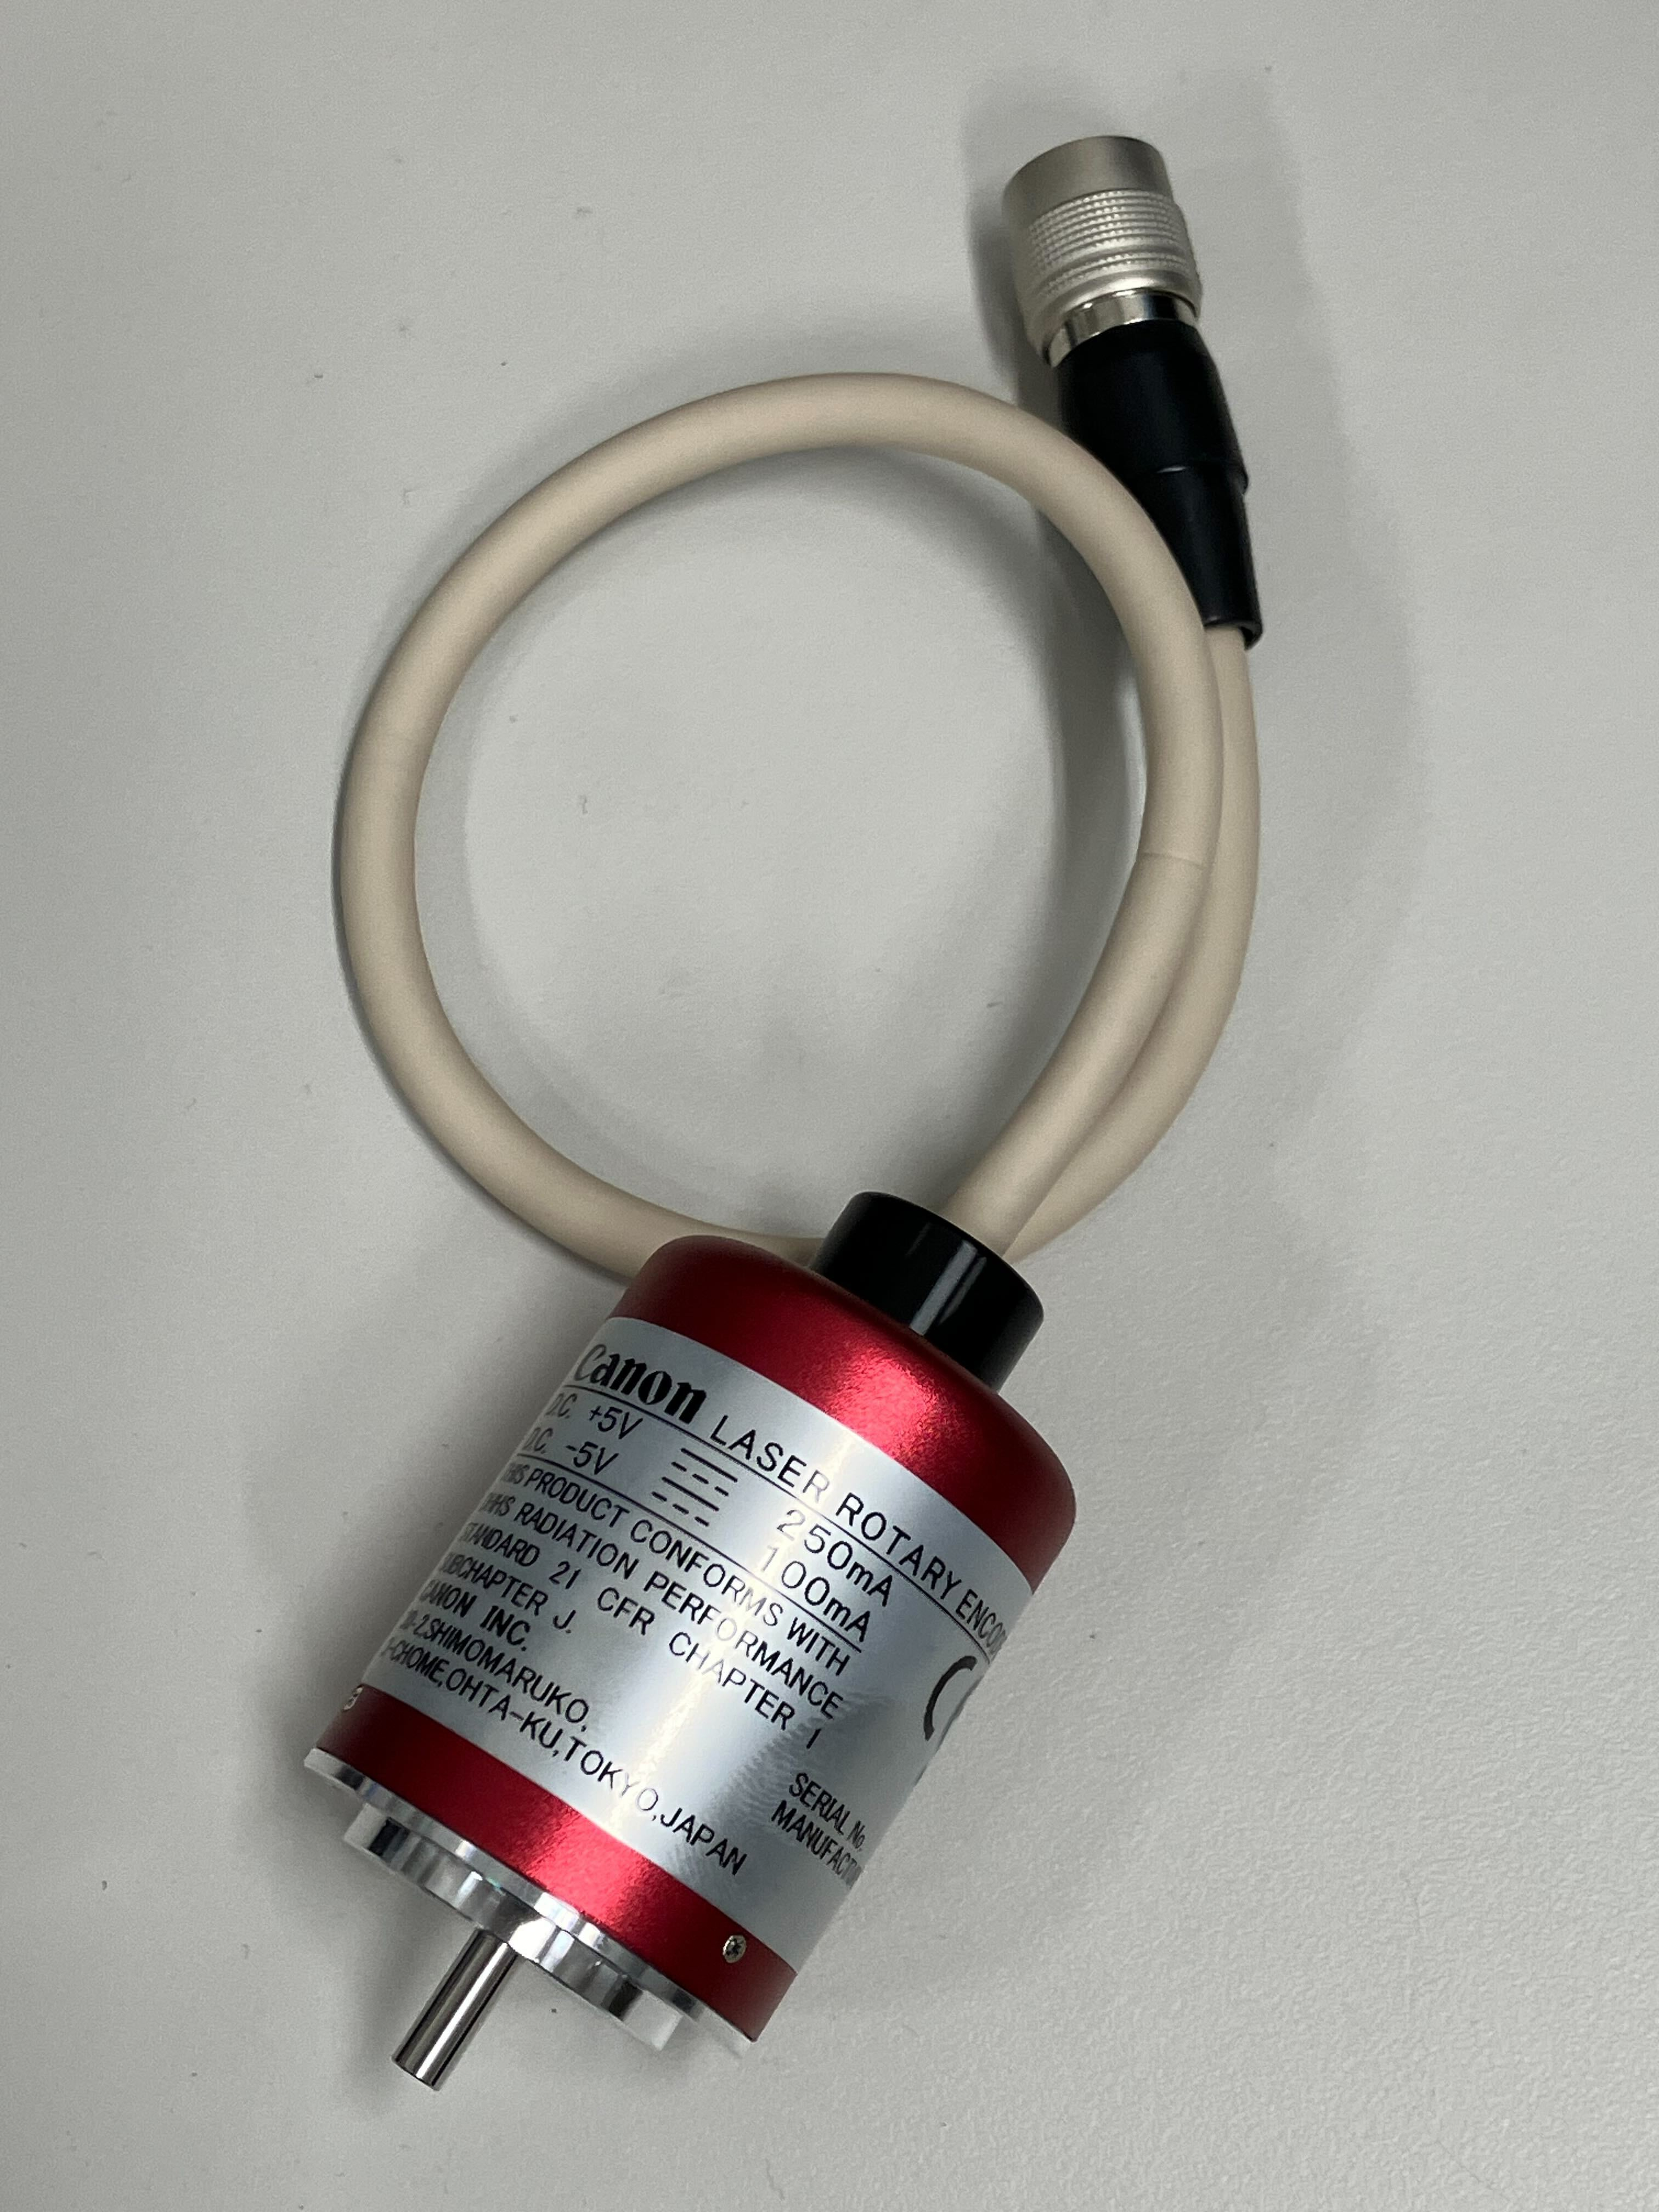
\includegraphics[keepaspectratio, scale=0.04]{4_elDAQ/figs/el_encoder.jpg}
      \subcaption{ロータリーエンコーダー(Canon, R-1SL \cite{R-1SL})}
    \end{minipage}
    %---- 2番目の図 --------------------------
    \begin{minipage}[t]{0.45\hsize}
      \centering
      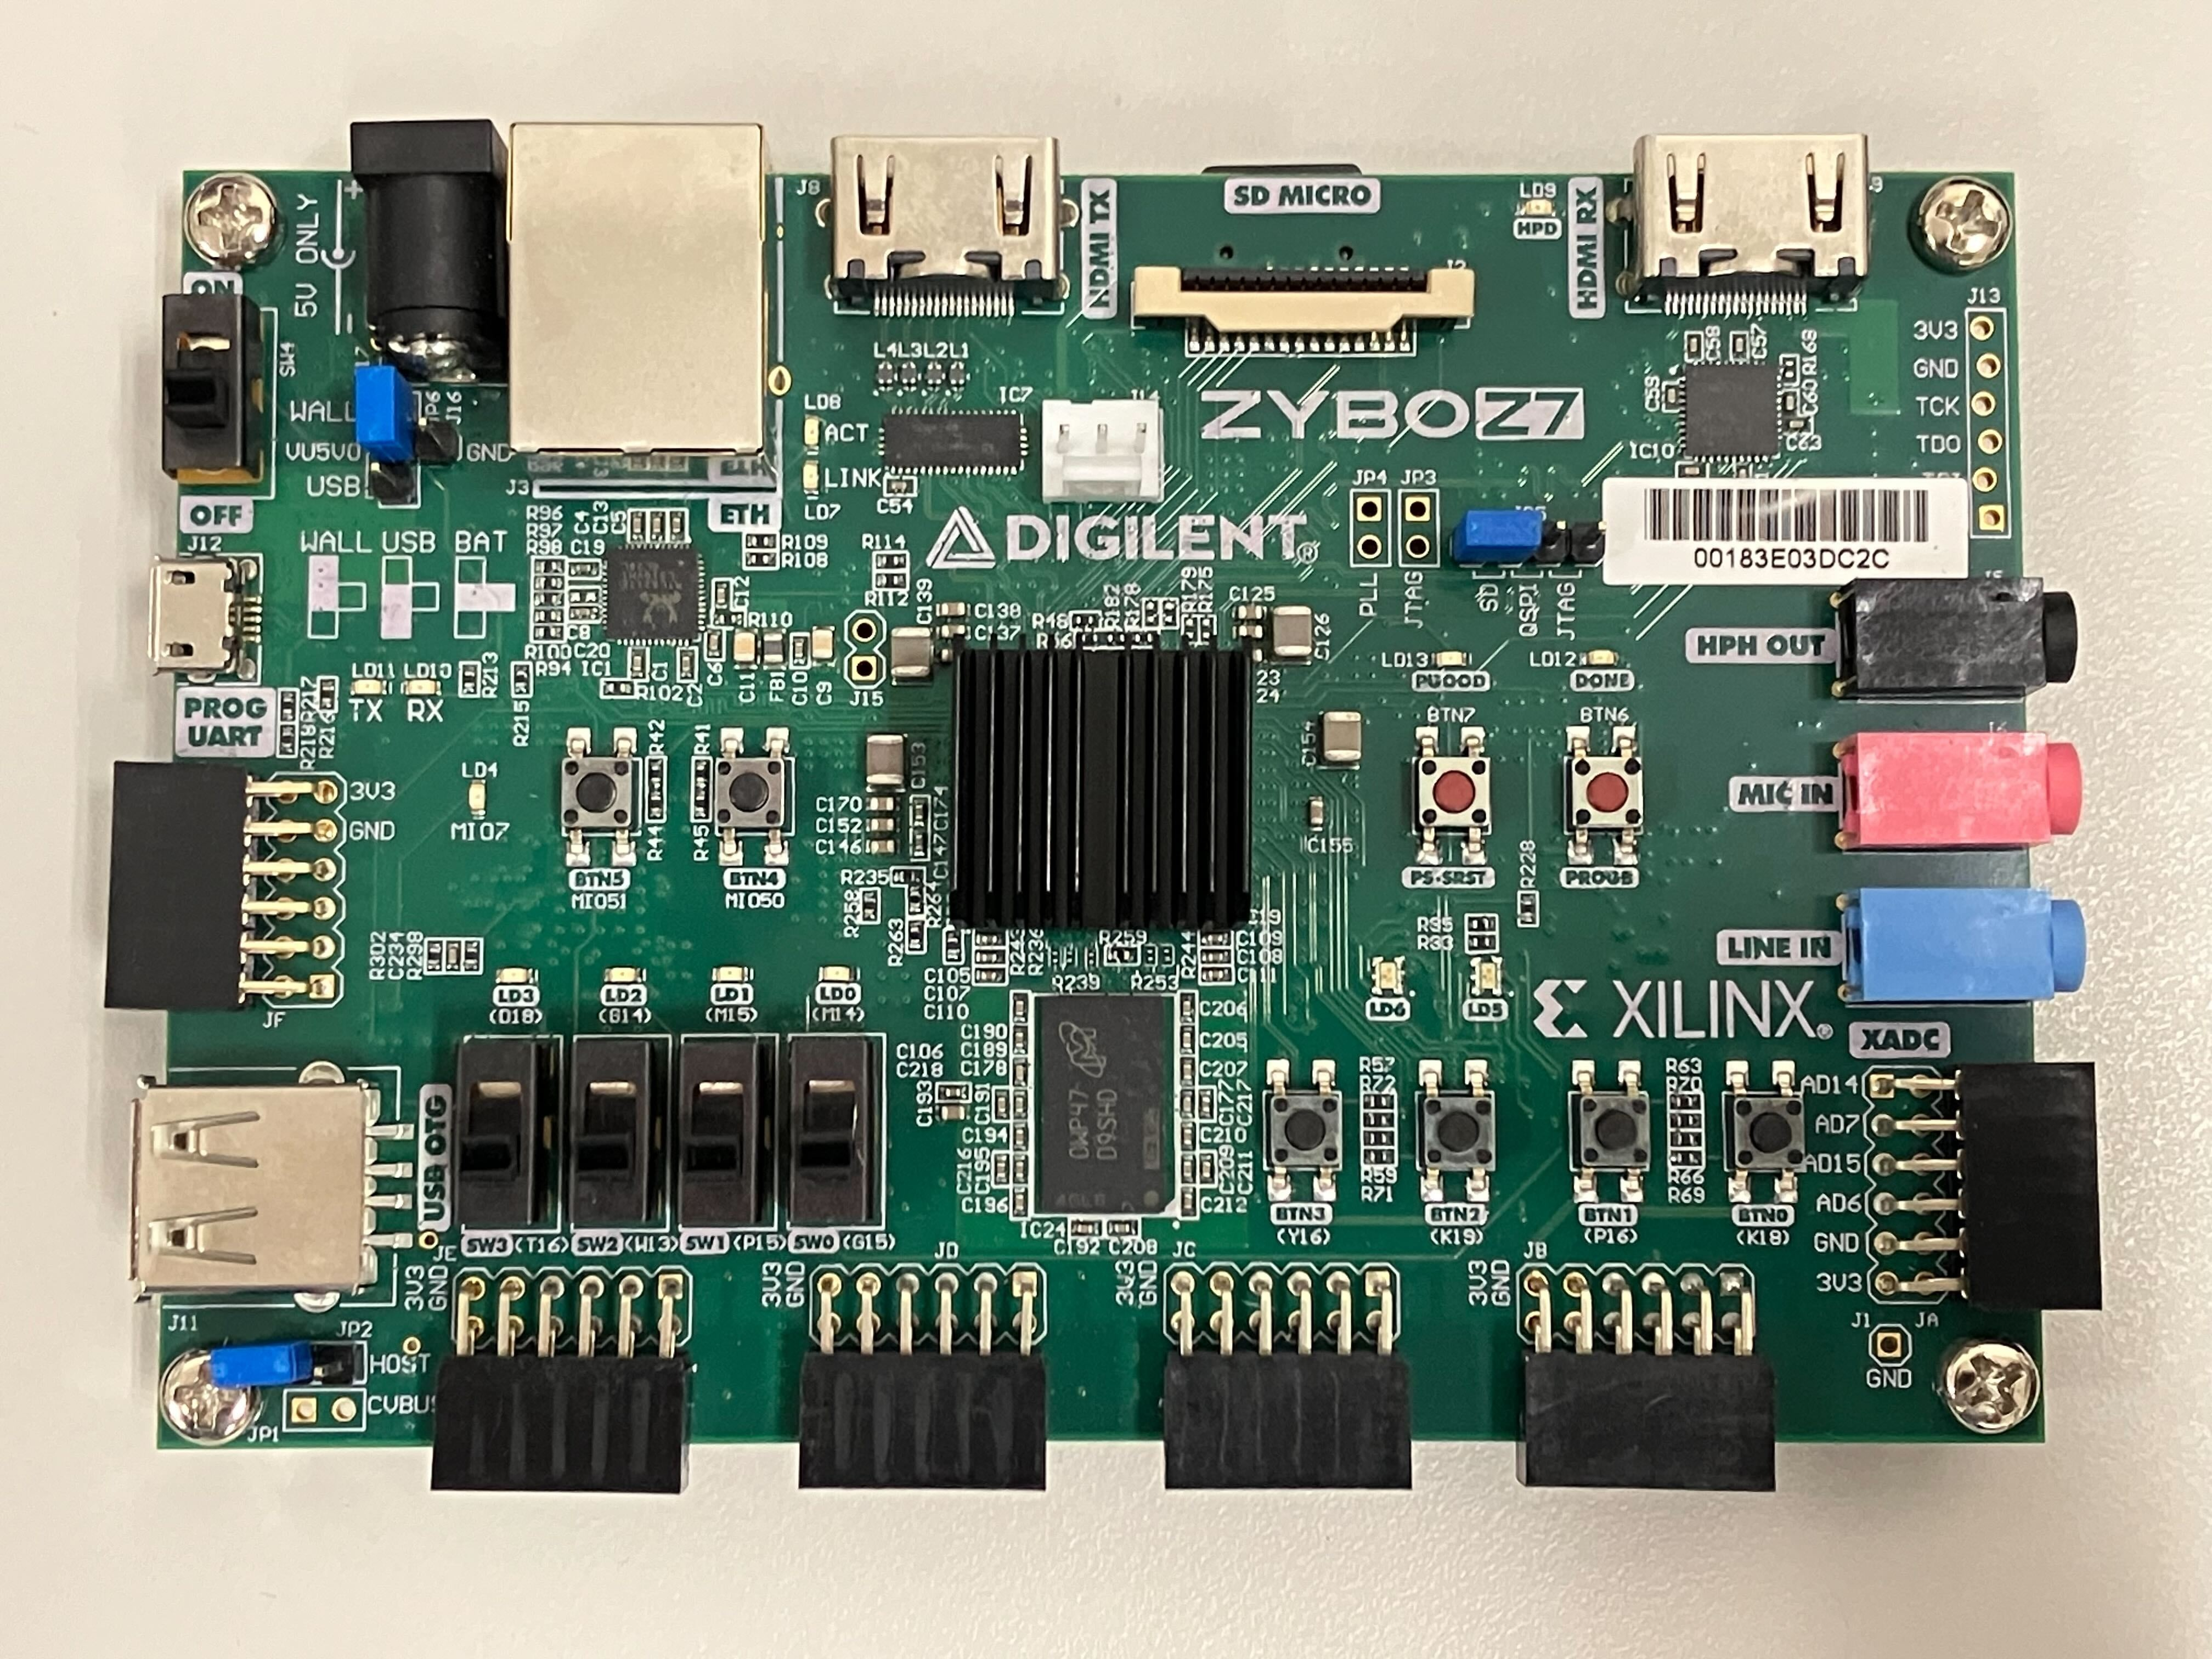
\includegraphics[keepaspectratio, scale=0.045]{4_elDAQ/figs/Zybo.jpg}
      \subcaption{FPGAボードZybo Z7-20 \cite{Zybo}}
    \end{minipage}
    %---- 図はここまで ----------------------
  \end{tabular}
  \caption{仰角方向の角度データ読み出し}
  \label{el_daq}
\end{figure}

方位角方向の角度データは、回転台下部に取り付けられたロータリーエンコーダー(HEIDENHAIN, ERM220 \cite{ERM220})を使用し、Xilinx製のFPGAボードSpartan3E \cite{Spartan}で読み出す(図\ref{az_daq})。エンコーダー自体の角度分解能は2.6分角($4.4\cdot {10^{-2}}^{\circ}$)である。さらに、平滑化フィルターを用いた方位角データの補完を行うことで、角度分解能を$5.7\cdot {10^{-2}}$分角($9.5\cdot {10^{-4}}^{\circ}$)に向上させている\cite{ikemitsu}。

\begin{figure}[h]
  \begin{tabular}{cc}
    %---- 最初の図 ---------------------------
    \begin{minipage}[t]{0.45\hsize}
      \centering
      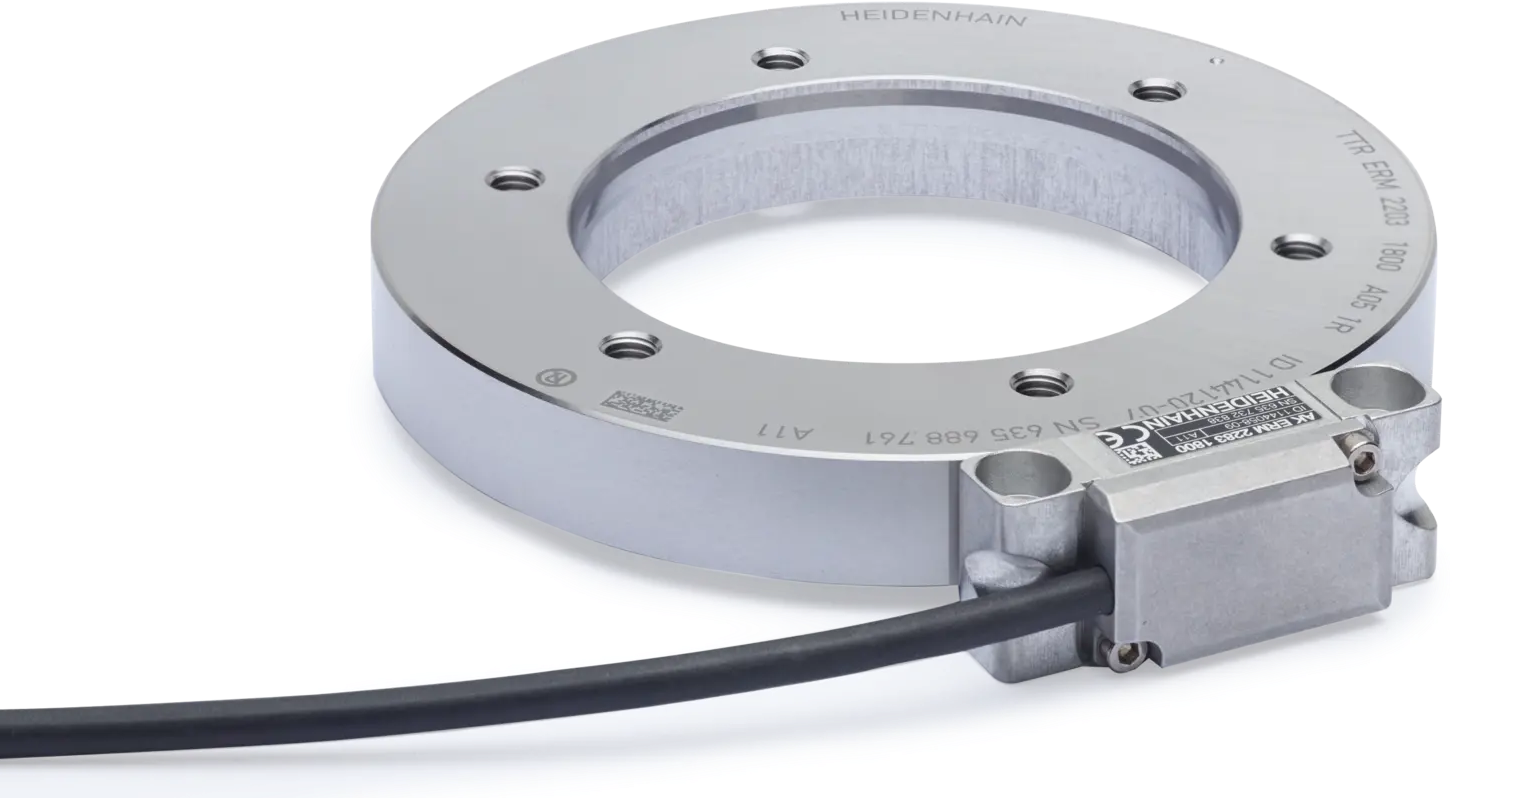
\includegraphics[keepaspectratio, scale=0.1]{4_elDAQ/figs/ERM220.png}
      \subcaption{ロータリーエンコーダー(HEIDENHAIN, ERM220 \cite{ERM220})}
    \end{minipage}
    %---- 2番目の図 --------------------------
    \begin{minipage}[t]{0.45\hsize}
      \centering
      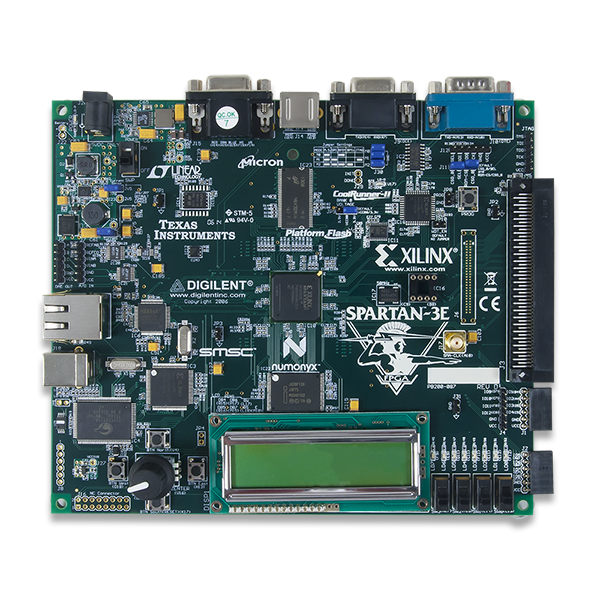
\includegraphics[keepaspectratio, scale=1.1]{4_elDAQ/figs/spartan-3e-2.png}
      \subcaption{FPGAボードSpartan3E \cite{Spartan}}
    \end{minipage}
    %---- 図はここまで ----------------------
  \end{tabular}
  \caption{方位角方向の角度データ読み出し}
  \label{az_daq}
\end{figure}

次に検出器のデータと方位角データに求められる同期精度を見積もる。時刻同期の精度を$\Delta t$とする。GroundBIRDの方位角方向の回転速度は最大で$120^{\circ}/s$になる。方位角方向での角度分解能$\Delta\phi$は
\begin{equation}
  \Delta\phi = 120^{\circ}/s \cdot \Delta t
\end{equation}
になる。時刻同期による角度の決定精度がエンコーダーの角度分解能よりも十分小さいことを課す。時刻同期による角度決定精度をデータ補完によって向上したエンコーダーの角度分解能である$9.5\cdot {10^{-4}}^{\circ}$の1\% 未満と要求すると、$\Delta t$の上限は
\begin{equation}
  \Delta t < \frac{9.5\cdot {10^{-4}}^{\circ}\cdot 0.01}{120^{\circ}/s} = 79 \text{ns}
\end{equation}
となる。この正確な時刻同期が必要になるため、仰角と方位角の角度データ読み出しで共にFPGAボードを使用している。先行研究 \cite{ikemitsu}により、時刻同期精度を55 ns に抑え、要求を満たす精度を実現している。

\begin{figure}[htbp]
  \centering
  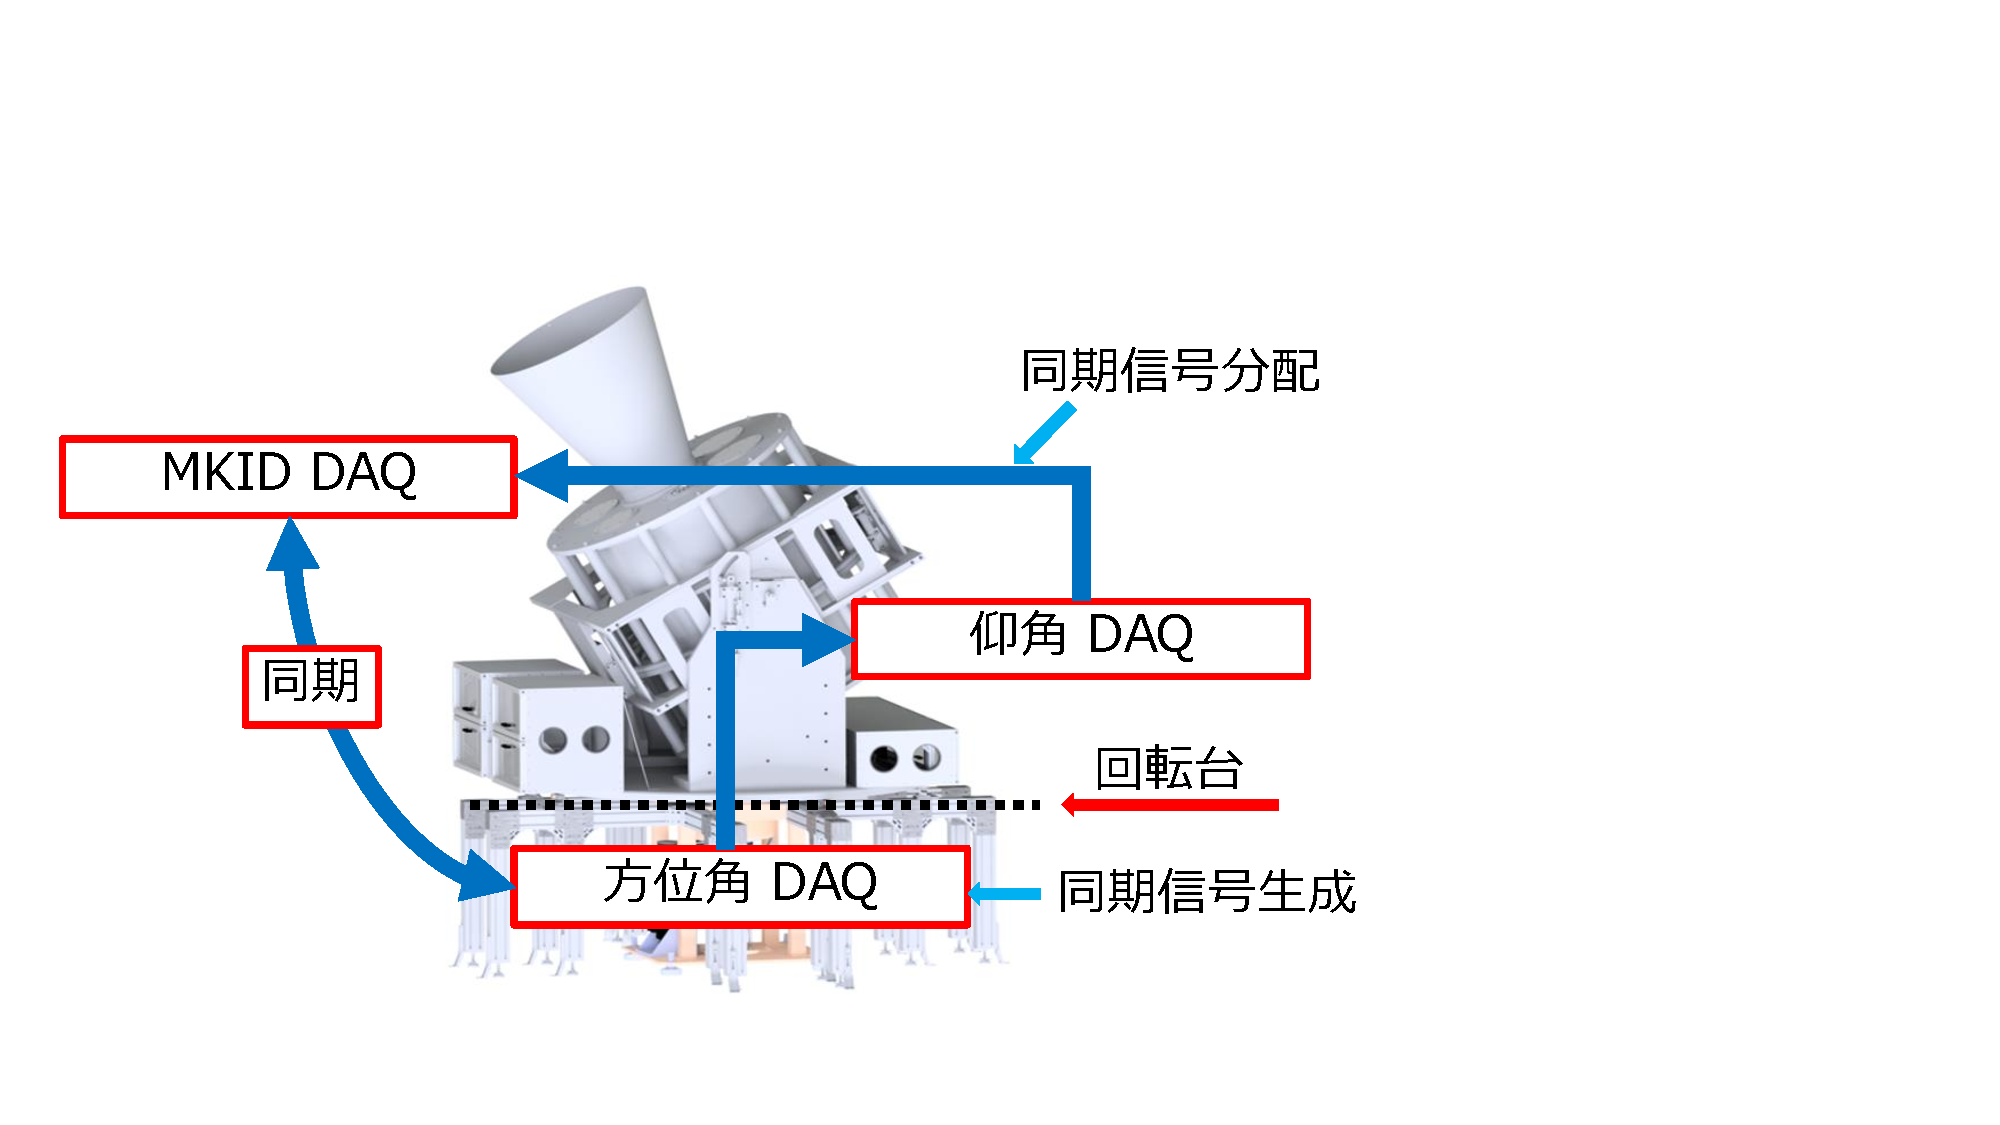
\includegraphics[width=0.9\columnwidth]{4_elDAQ/figs/GB_sync_2.pdf}
  \caption{GroundBIRDの同期信号の流れ。回転台下部の方位角DAQボードで生成された同期信号が回転継手を介して回転台上部のMKIDのDAQボードに送信される。その際、仰角DAQボードで同期信号を分配している。}
  \label{GB_sync}
\end{figure}

GroundBIRDでの同期信号の流れを説明する(図\ref{GB_sync})。望遠鏡が連続回転するため、回転台の上下の電気的な接続に同軸ケーブルのような通常の信号線は使用できない。そのため、回転継手を介して回転台上下での信号を共有している。また、回転台の上下のデータ取得系でレートの遅い``同期信号''を回転継手を介して共有することで時刻の同期を図っている。

同期信号によるデータ同期を次のステップで行なっている。
\begin{enumerate}
  \item 回転台下部の方位角DAQボードから1秒に1回、基準となる同期信号を出力する。
  \item 回転継手を介して回転台上部に届いた同期信号を仰角DAQボードに入力する。
  \item 回転台下部では、同期信号を出力した時刻情報を方位角のエンコーダーデータと共に保存する。
  \item 仰角DAQボード同期信号を分配し、検出器のDAQボードに送る。
  \item 同期信号の到達した時刻情報を検出器のTODと共に保存する。
  \item 2種類のTODの時刻情報を用いて、各時刻での検出器信号と角度データの同期を行う。
\end{enumerate}

\subsection{仰角データ取得における問題点}
本論文の研究対象である仰角のデータ取得に関して詳細に説明する。仰角のデータ取得系が担う役割は以下の2つである。
\begin{itemize}
  \item 仰角の角度データを取得する
  \item 同期信号の分配
\end{itemize}

\begin{figure}[htbp]
  \centering
  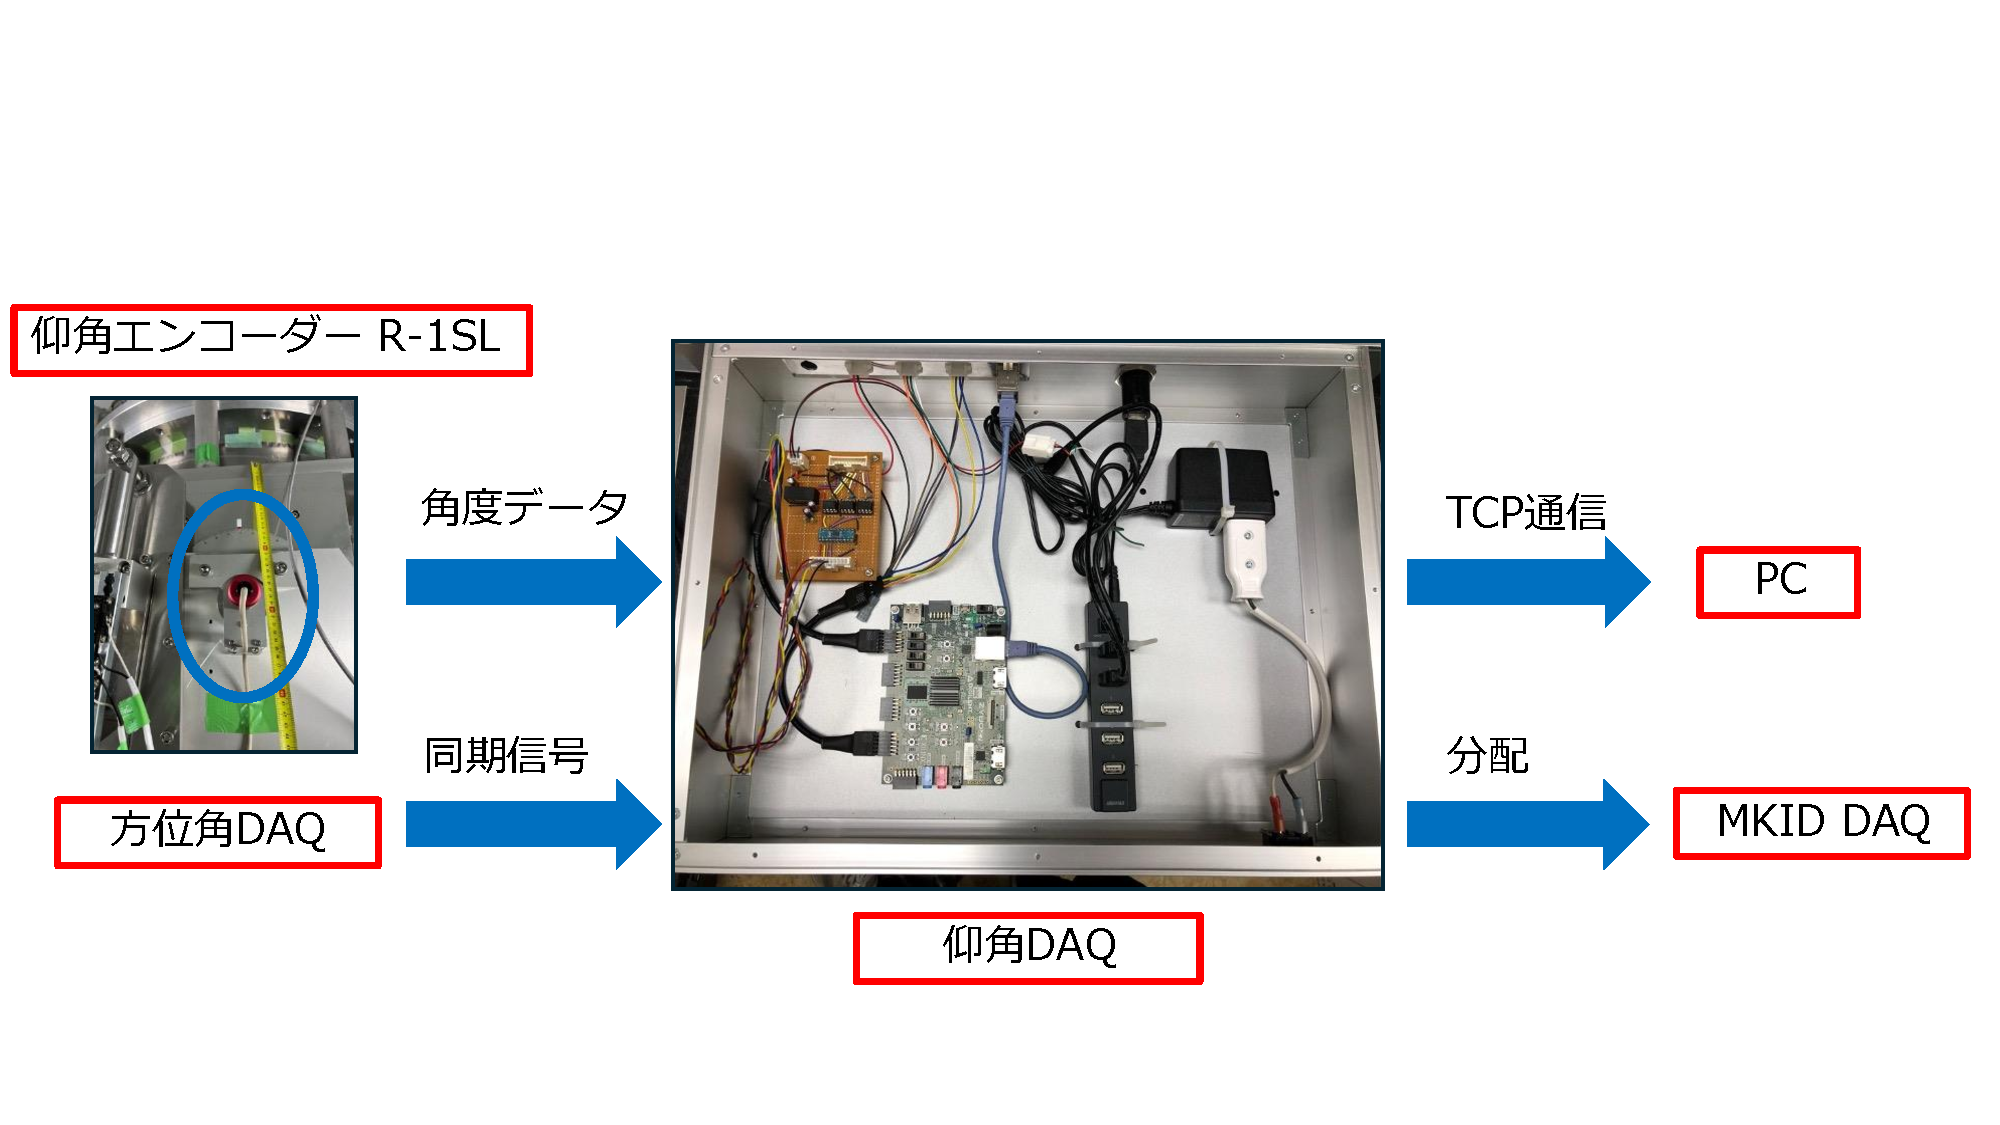
\includegraphics[width=1.0\columnwidth]{4_elDAQ/figs/el_daq_box.pdf}
  \caption{仰角データ取得システムの全体像。信号処理のほぼ全てをZybo \cite{Zybo}が担う。信号の電圧変換、Zybo、電源からなるコンパクトなデータ取得系は1つのボックス内に配置されている。}
  \label{GB_daq_box}
\end{figure}

データ取得系は非常にコンパクトであり(図\ref{GB_daq_box})、信号の処理はZybo内に搭載されている``Zynq \cite{Zynq}''と呼ばれるチップで行っている。ZynqはXilinxが開発した、CPU、FPGAなどが1チップに統合されたSystem on Chip (SoC)の1つである。ZynqはCPUを搭載するProcessing System (PS)部分と、FPGAを搭載するProgrammable Logic (PL)部分に大きく分けられ、FPGAが得意とする並列処理や高速処理と、CPUが得意とする複雑な処理とで役割を分担できるため、効率の良い処理が可能となる。先行研究でFPGAに搭載するファームウェア\footnote{FPGAに組み込む機能を本論文ではファームウェアと呼ぶことにする。}の開発がなされており、実装されている。

\begin{figure}[htbp]
  \centering
  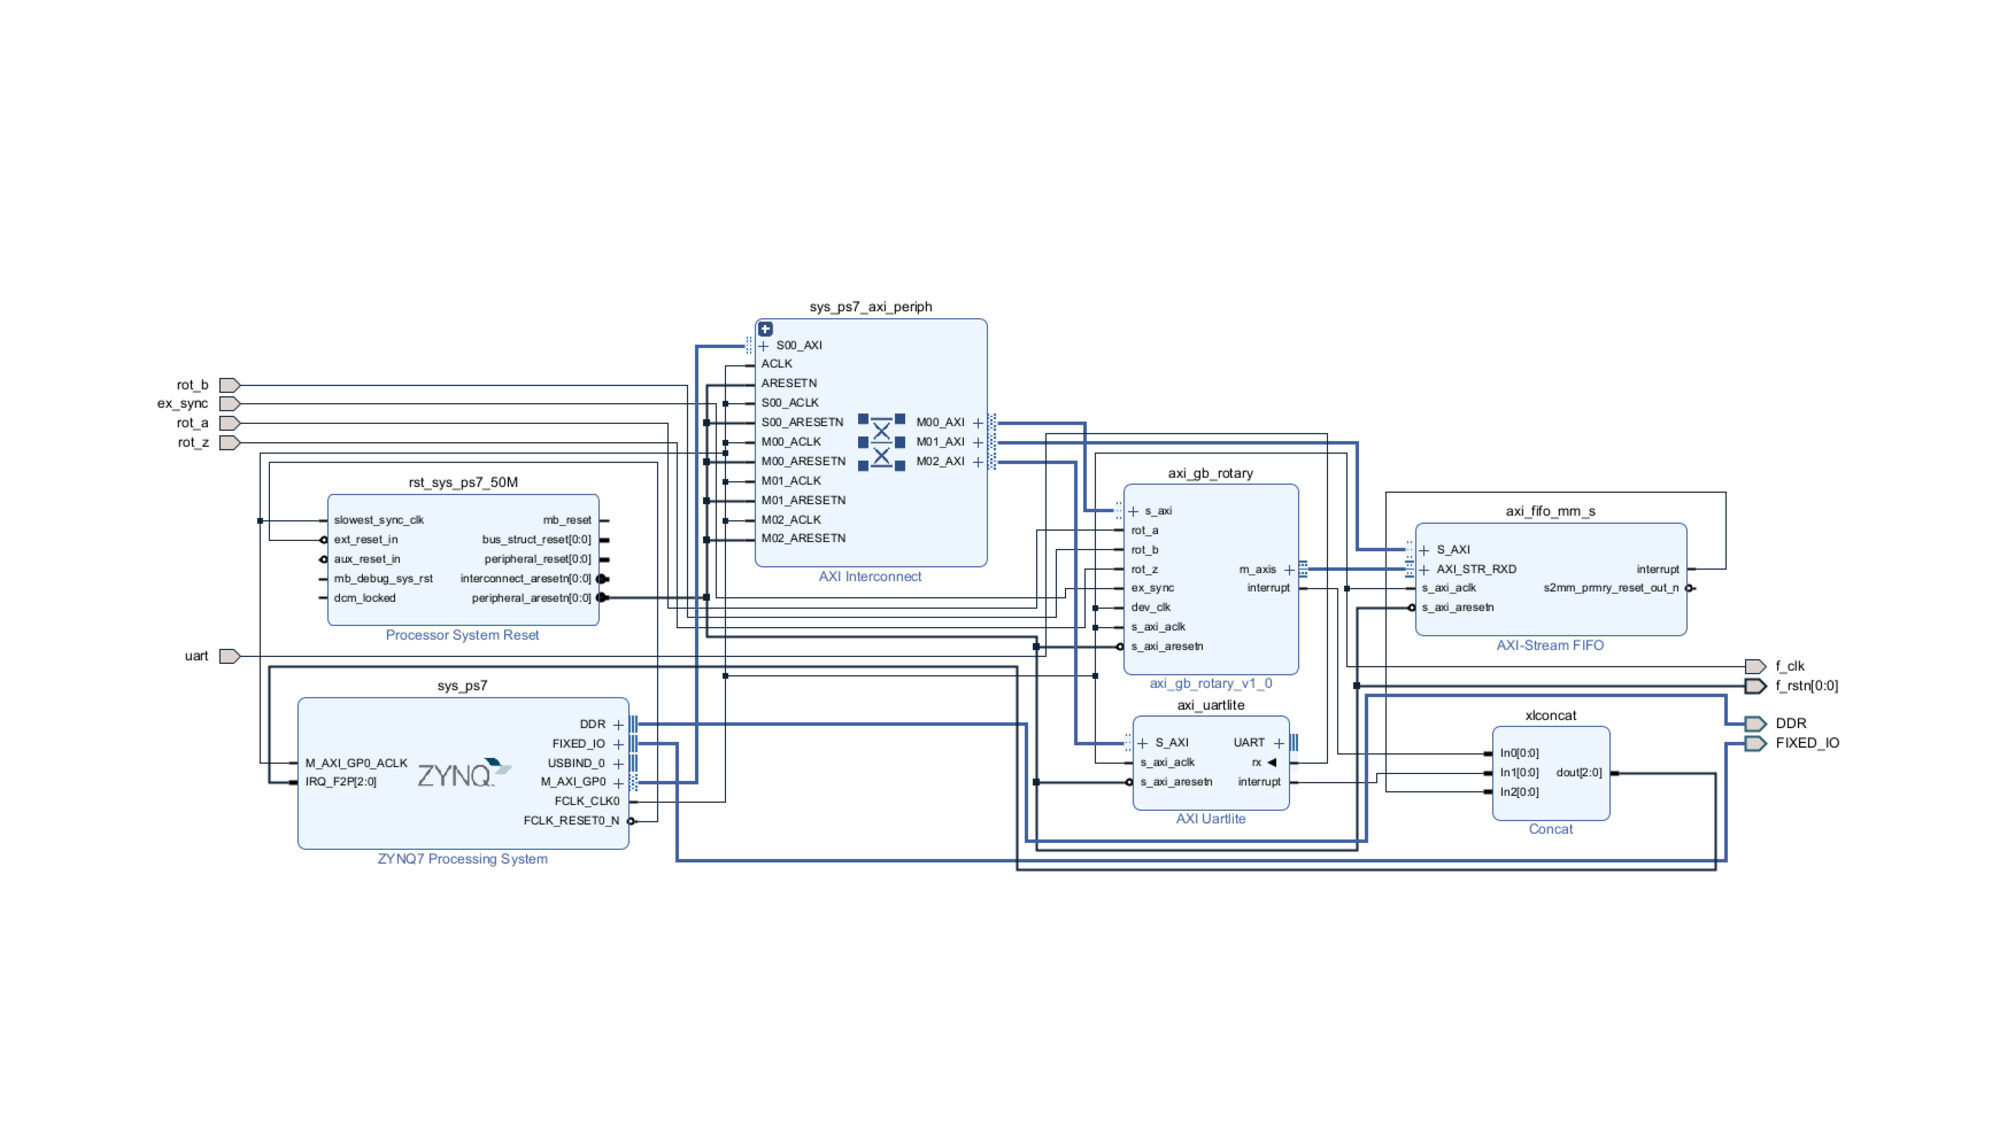
\includegraphics[width=1.0\columnwidth]{4_elDAQ/figs/block_diagram.pdf}
  \caption{IPインテグレータの配線図。青く囲まれているブロックがIPコアを表す。ブロックの左側から出る線が入力信号で、右側から出る線が出力信号になっている。図中の``axi\_gb\_rotary''と呼ばれるIPが自作IPで、デコーダーの役割を担っている。}
  \label{block_diagram}
\end{figure}

FPGA上でのファームウェアの全体図を図\ref{block_diagram}に示す。設計にはVivadoというXilinx製の開発ソフトを用いる。様々なIPコア(機能ごとの回路のまとまり)をIPインテグレータというGUI上で配線し、全体のファームウェアを構成する。IPは自作のIPと、Xilinx製のIPを組み合わせて使用している。

\begin{figure}[htbp]
  \centering
  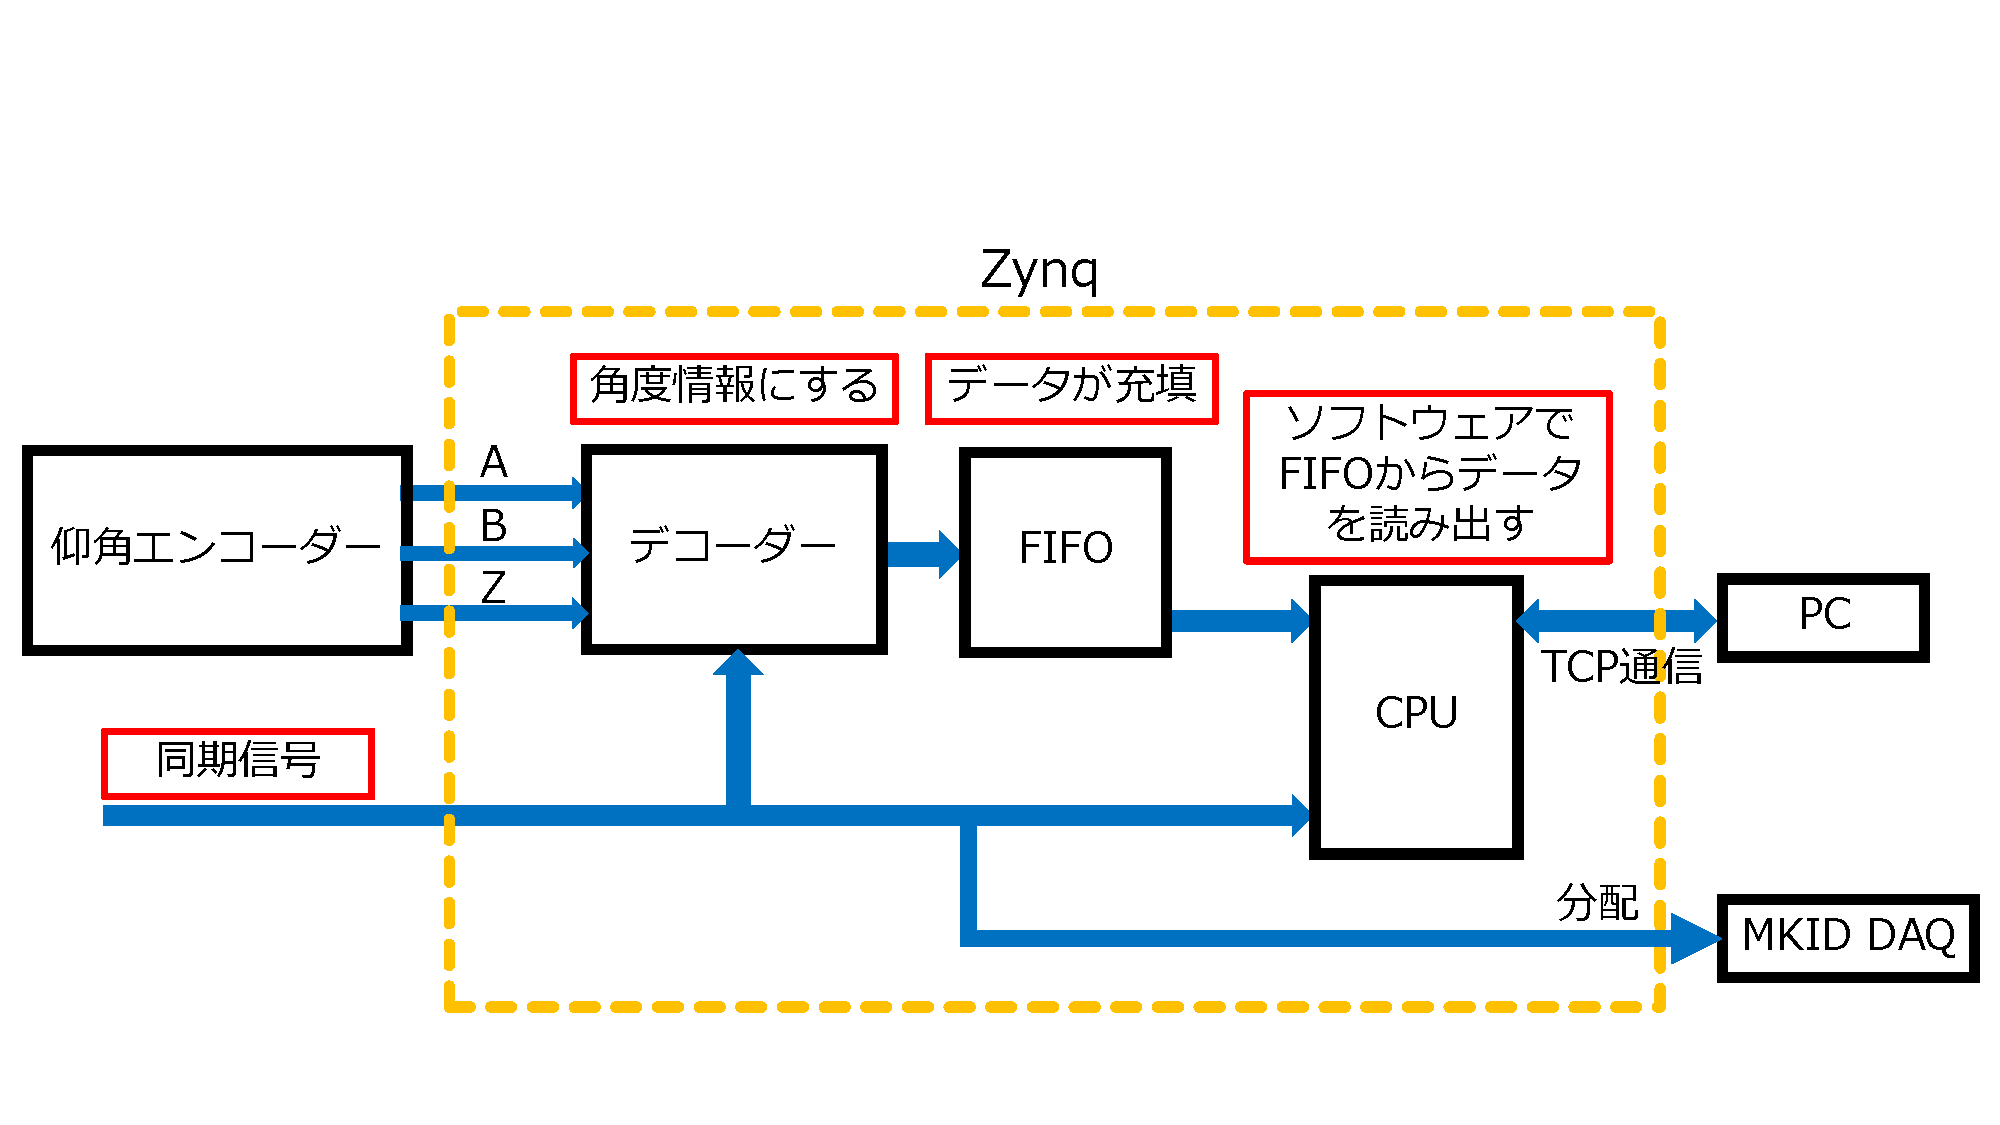
\includegraphics[width=1.0\columnwidth]{4_elDAQ/figs/zynq_flow.pdf}
  \caption{Zynq内での信号処理。エンコーダーからの角度データ処理と方位角DAQボードからの同期信号の分配を1チップ内で行う。}
  \label{zynq_flow}
\end{figure}

Zynq内での処理の模式図を図\ref{zynq_flow}に示す。仰角エンコーダーはインクリメンタル方式を採用しており、エンコーダーからの出力信号は A相、B相、Z相の3相からなる。エンコーダーからの出力パルス数で角度の変化量、A相とB相のパルスの立ち上がり順で回転方向が分かる仕様になっている。また、Z相信号は1回転で1度出力され、回転の原点として使用される。3相の信号はZynq内のデコーダー部分で角度情報として翻訳され、1kSPSで``FIFO \cite{FIFO}''に充填される。FIFOとはfirst-in first-outメモリのことで、データを格納し、取り出す際は、格納した順番通りに先に格納したデータから取り出す構成になっている。FIFOに格納されたデータはCPUのソフトウェアで読み出し、TCP通信でPCへと送信される。

同期信号の通信方式はUART\footnote{UART通信では、送信側と受信側で通信速度を決めておき、1byte (8bits)ずつ情報のやり取りを行う。1byteのまとまりでは、``start bit (1bit)''、``data (8bits)''、``parity bit (1bit、情報の誤検知に使用)''、``stop bit (1bit)''の4つで構成され、全11bitsになる。}を使用しており、デコーダー部分でタイムスタンプ(測定開始時からの経過時間)情報を取得する。また、MKIDのDAQは複数のボードを使用するため、同期信号を分配させ、送信している。

\begin{figure}[htbp]
  \centering
  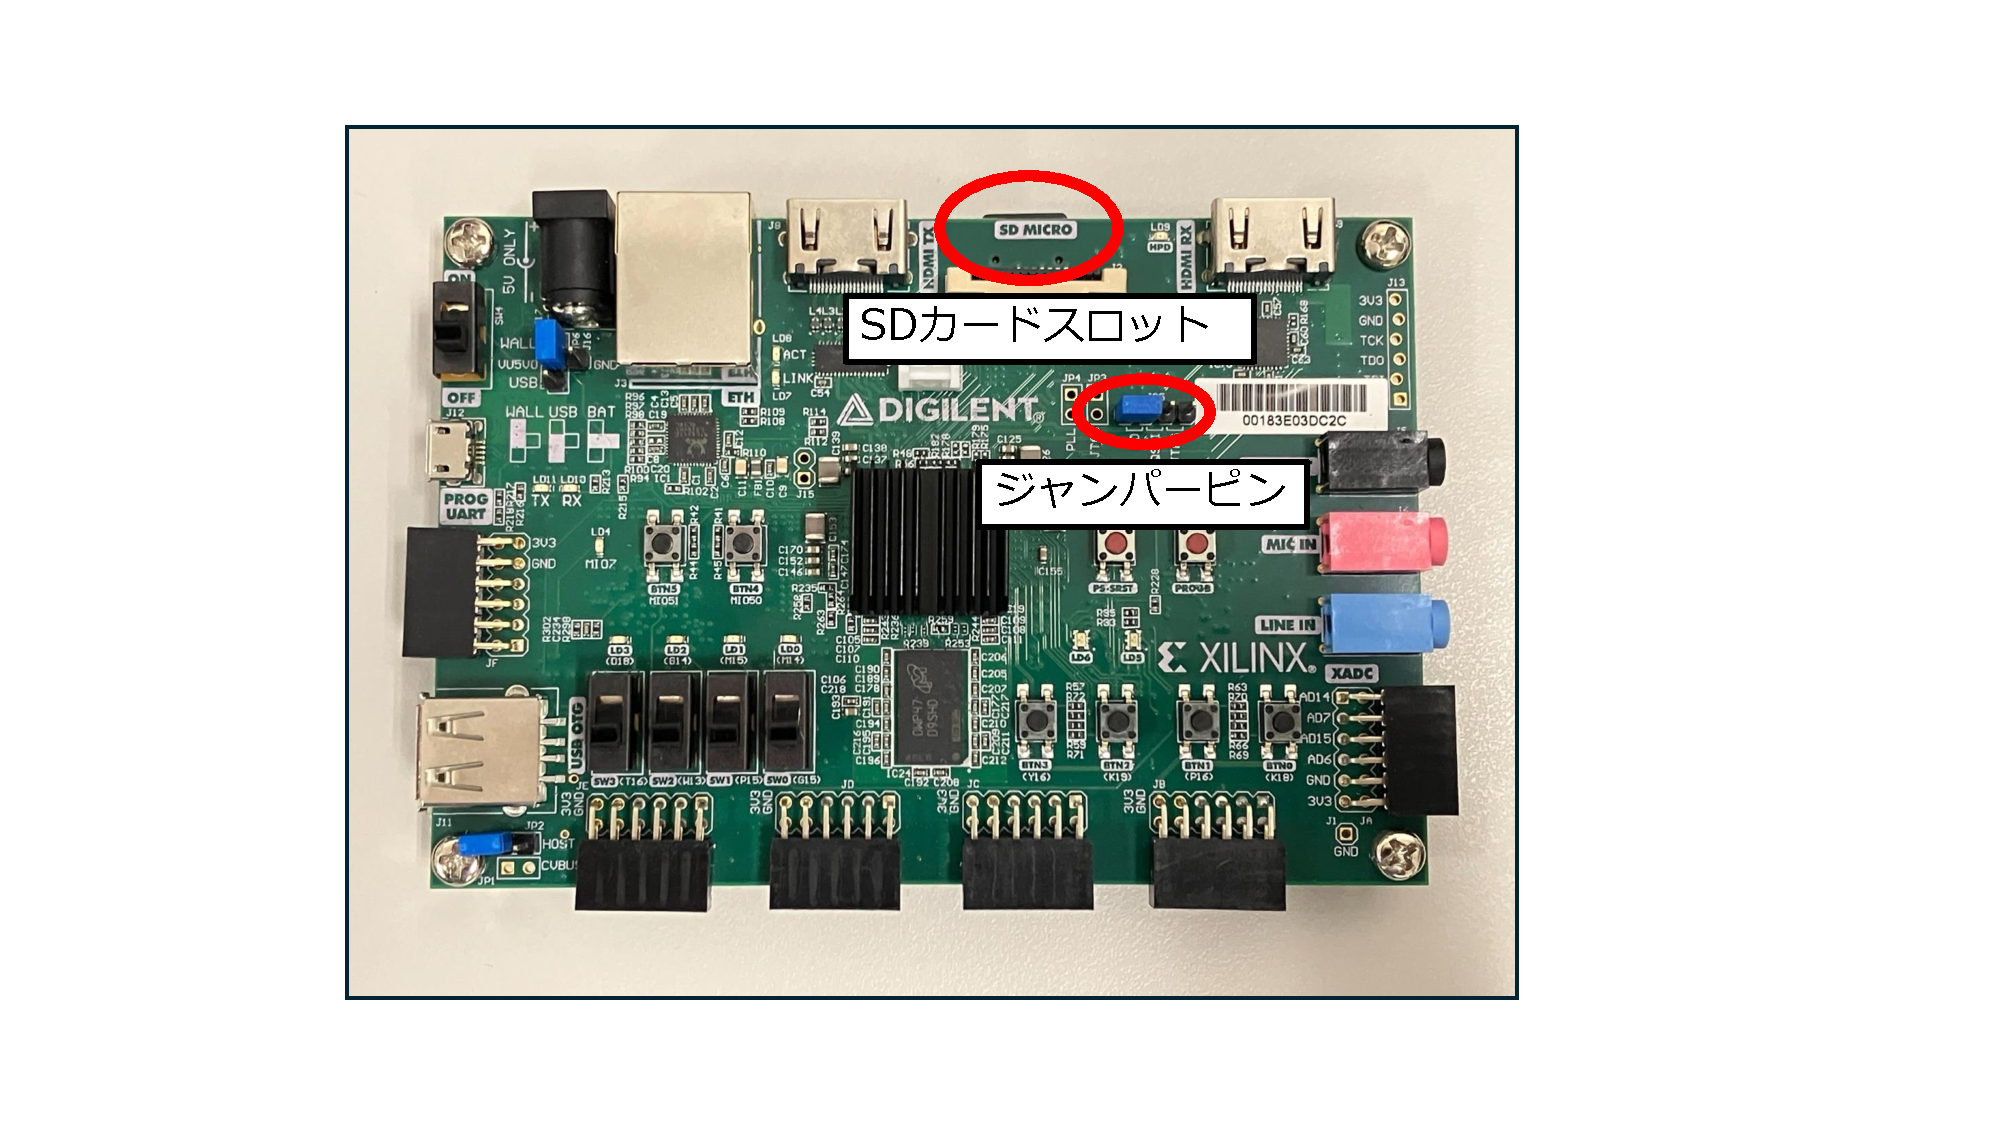
\includegraphics[width=0.6\columnwidth]{4_elDAQ/figs/sd_zybo2.pdf}
  \caption{ZyboにはSDカードスロットが付いている。システムを起動するために必要なファイルをSDカードに書き込み、スロットに差し込んで電源を入れることで稼働が開始する。ジャンパーピンはSDに設定しておく。}
  \label{sd_zybo}
\end{figure}

以上の構成で仰角DAQシステムを稼働させていた(図\ref{sd_zybo})が、観測の長期運用を考えた際に、問題点を抱えていた。Zynqでのデータ処理とPCへの通信をOSのない(ベアメタル\footnote{本来は「剥き出しの金属」という意味だが、転じてOSがインストールされていないコンピュータのことを指す。})環境でソフトウェアを動かすことで行っている。このことにより、システム全体が硬直的になっており、その扱いにおいて柔軟性がない。柔軟性がないことで起きる問題として以下のものが挙げられる。
\begin{itemize}
  \item データ取得が異常終了した際のメンテナンスが難しい
  \item OSが介さない通信による信頼性の低下
  \item ソフトウェア、FPGA面での改良が難しい
\end{itemize}

最も大きな問題はメンテナンス性である。観測の有無に問わず、望遠鏡の角度データは常に取得し続けており、安定した仰角データ取得が必要不可欠である。しかし、仰角エンコーダーからPCまでのデータの流れが途切れてしまうことがある。それは、通信のエラーや停電等による電源系統の不具合など様々な要因からくるもので、長期運用をする上ではある程度避けられないものである。その際、エンコーダーとZybo間の通信が切れて、Zynq内でのエンコーダー情報が失われる。加えて、エンコーダーの原点情報も失われるため、通信を再開させた際に読み出した角度の値にオフセット値が乗ってしまう。Zynq内で原点情報を記憶させるには望遠鏡の仰角を動かし、エンコーダーのZ相信号を取得して値をリセットすることが必要であり、手間のかかる工程になる。この一連のメンテナンスをまとめると以下のステップに分けられる。
\begin{enumerate}
  \item Zyboを再起動させて再度ソフトウェアを動かす
  \item 望遠鏡の仰角を動かしてZ相信号を入力し、原点情報を記憶
  \item 仰角を$70^{\circ}$まで動かして固定
\end{enumerate}

この中で、Zyboの再起動と仰角を動かす際にケーブルに変な張力がかかっていないかの目視に現地での作業を要する。リモートでの望遠鏡運用を進める上で、少しでも現地で必要な作業を減らし、リモートでメンテナンスができることが望まれる。

また、ZyboとPCとのTCP通信を行うために、ベアメタル環境ではTCP/IPのプロトコルスタックを独自で実装しなければいけない。今回は``lwIP(lightweight IP)''と呼ばれるオープンソースのTCP/IPプロトコルスタックを使用してTCP通信を実装している。そのため、通信に関わるソフトウェアが複雑化する上、OSが通信を取り仕切るよりも信頼性に欠ける。

加えて、システムに組み込まれたソフトウェアやFPGAのファームウェアは固定化されており、今後の運用で変更点が生じた時に、SDカードに新しいファイルシステムを書き込んで全面的にシステム更新しなければならず、労力を要する。システムのカスタマイズ性を上げ、変更を容易にできるようになれば、運用に関わるコストを削減することができる。

\subsection{PYNQを用いた新システムの導入}
上に述べた問題を改善するために、本研究では既存のZynqシステムにOSを搭載し、ソフトウェアをOS上で動かすことでシステム全体の柔軟性向上を試みた。これにより上記の問題点に対して
\begin{itemize}
  \item データ取得が異常終了した際のメンテナンスをリモート主体で行える
  \item OSが通信を介すことで信頼性が向上
  \item ソフトウェア、FPGA面での改良をシステムを起動したまま行える
\end{itemize}
という改善が期待できる。一方でベアメタル環境に比べてOSをインストールすることで実行時間と使用メモリが増えるが、FIFOへのデータ充填とFIFOからの読み出しはともに1kSPSであり、FIFOの容量も十分であるため、性能に問題は出ない。Zynqに搭載するOSは基本的にlinuxベースであるが、今回は``PYNQ \cite{Pynq}''と呼ばれるUbuntu\footnote{今回はUbuntu 22.04がベースになっている}、JupyterおよびPythonをベースとしたフレームワークを搭載した。PYNQを採用した理由として
\begin{itemize}
  \item ソフトウェアをPYNQ上のPythonスクリプトで動かせるため、通信スクリプトを簡潔に記述できる
  \item システム起動に必要なブートイメージファイルの作成が容易
  \item ``Overlay''と呼ばれる機能を使用することでFPGAのファームウェアをPythonで容易に変更できる
\end{itemize}
が挙げられる。

ここでPYNQのイメージファイル作成の概要を説明する。基本的な手順は\cite{image}を参考にし、作業環境はDocker上のUbuntu 20.04で構築した。その際に使用した開発ツールとバージョンを表\ref{PYNQ_table}にまとめる

\begin{table}[htbp]
  \centering
  \caption{PYNQイメージ作成で使用したツールとバージョン}
  \vspace{3mm}
  \begin{tabular}{cc} \hline
    ツール & バージョン \\ \hline
    Vivado & 2022.1\\
    PYNQ linuxイメージ & 3.0.1\\
    PetaLinux & 2022.1\\ \hline
  \end{tabular}
  \label{PYNQ_table}
\end{table}

PetaLinuxとはXilinxが提供する、ZynqをはじめとするSoC用のlinuxシステムをビルドするためのツールである。この環境のもとで以下のステップでPYNQイメージを作成した。
\begin{enumerate}
  \item ベースとなるFPGAファームウェアの作成
  \item Zybo用のスペックファイルの作成
  \item ビルド
\end{enumerate}

FPGAファームウェアはOverlayによってZybo起動時に変更できるため、この時点では最も単純な回路をVivadoで準備してやれば良い。それをもとにVivado上でコンパイルをし、生成された4つの回路情報を持つファイル(.xsaファイル、.bitファイル、.hwhファイル、.tclファイル)を取得する。

スペックファイルはZyboのスペック情報を.specファイルとして作成する。その後、作成した全ファイルをビルド用のディレクトリに置く。最後にmakeを実行してビルドを行い、PYNQイメージファイル(.imgファイル)を生成して完了する。

このイメージファイルをSDカードにddコマンド等で書き込み、ZyboのSDカードスロットに差し込むことでPYNQが起動する。また、起動時にOverlayスクリプトを走らせて図\ref{block_diagram}で示したファームウェアでFPGAの回路を上書きするように設定した。これにより、本来の回路情報がPYNQ上で再現される。Overlayを用いてFPGAのファームウェアを変更する仕組みを図\ref{overlay}に示す。

\begin{figure}[htbp]
  \centering
  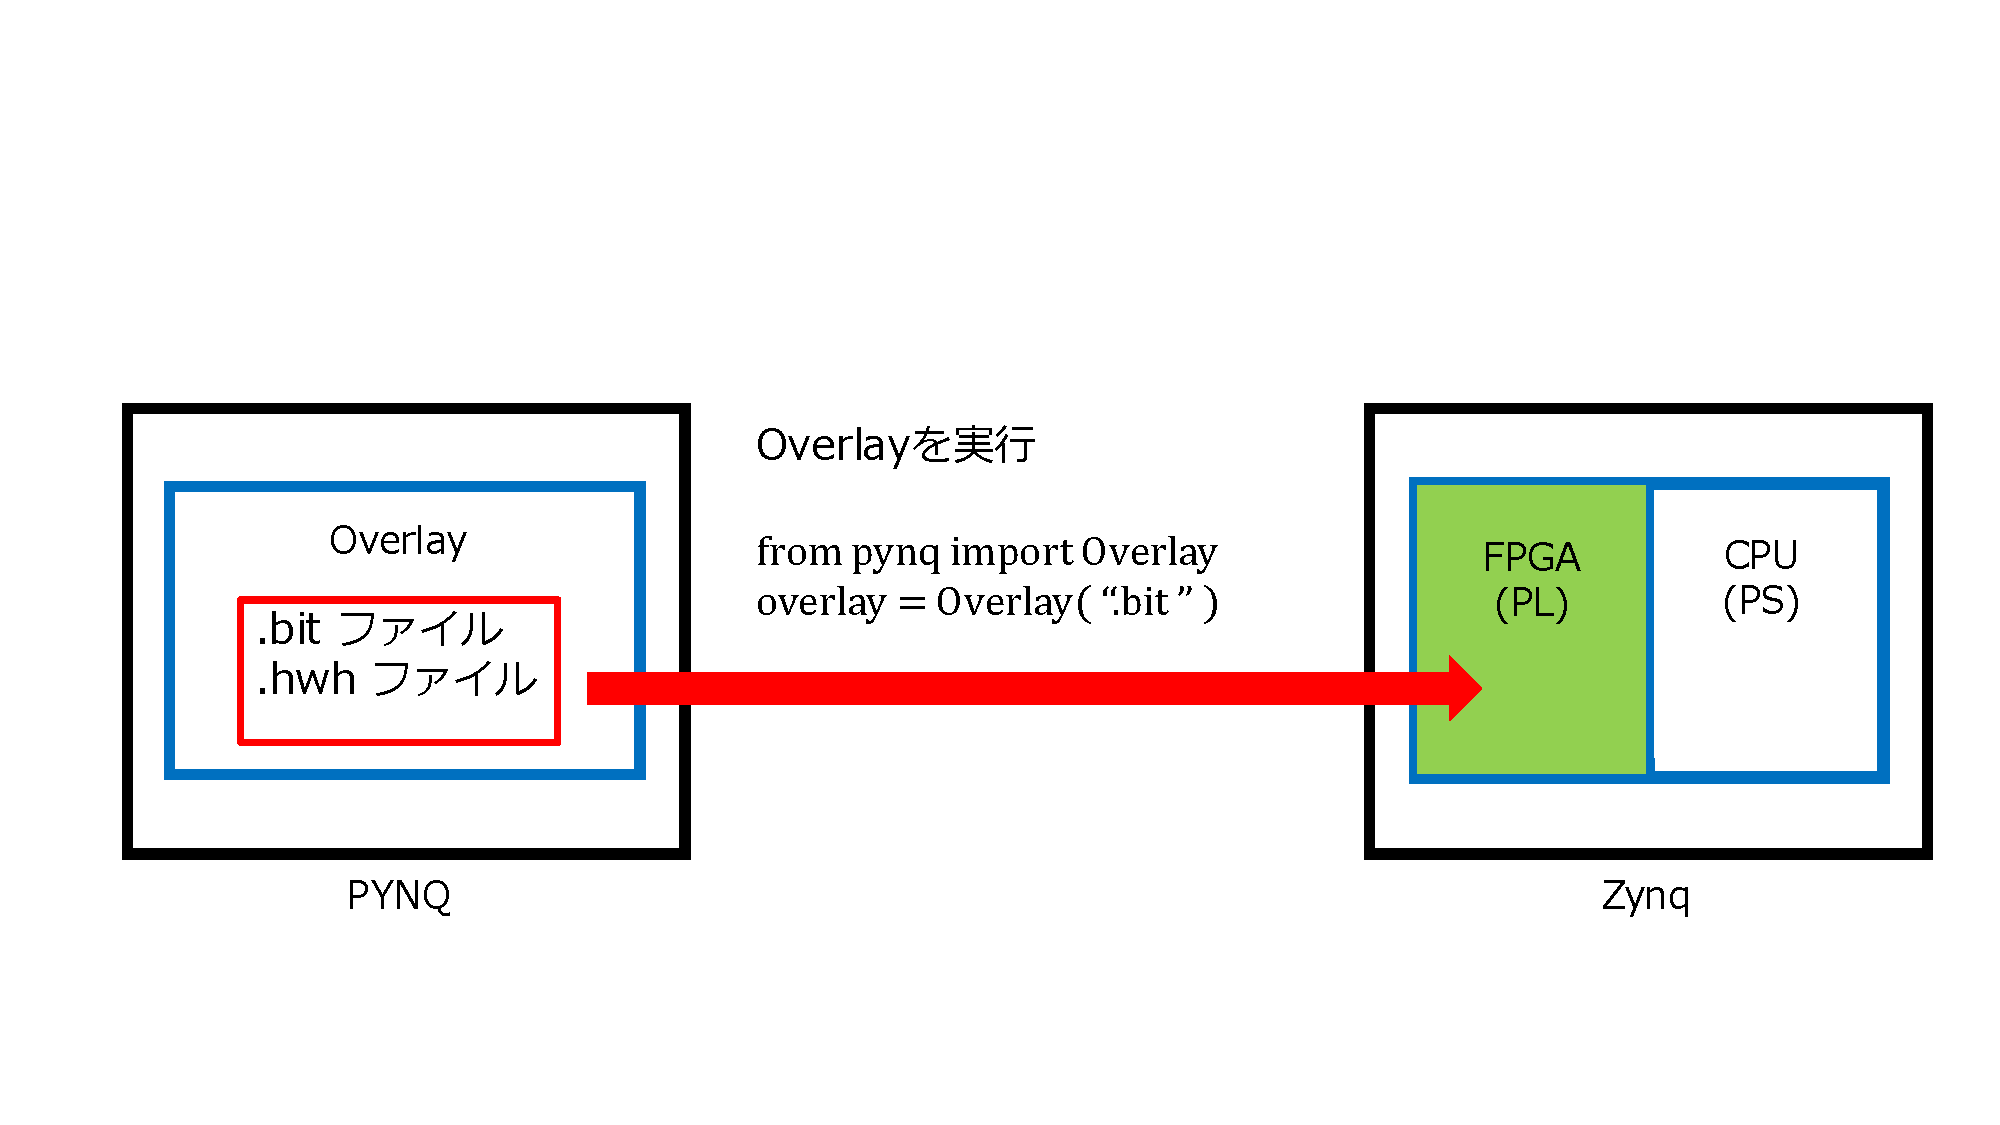
\includegraphics[width=1.0\columnwidth]{4_elDAQ/figs/overlay3.pdf}
  \caption{PYNQからFPGAのファームウェアを変更する模式図。Vivadoで設計した新しい回路ファイルをOverlayクラスに読み込ませることで容易に変更ができる。}
  \label{overlay}
\end{figure}

Overlayに必要なファイルはVivadoでコンパイルをして生成される.bitファイルと.hwhファイルの2つである。これらは同じディレクトリに置いておく。PythonでOverlayクラスをインポートし、.bitファイルを読み込ませることでOverlayは実行される。その際、Overlayクラスは同じディレクトリにある.hwhファイルも読み込んでくれる。図で示したようにOverlayスクリプトはたった2行で書くことができ、ファームウェアの変更は非常に容易に実行できる。

最後に、Zynq内で動かすスクリプトをPYNQ用にPythonで再構築した。

\section{望遠鏡への実装}

\subsection{新データ取得システムのインストール}
新しく導入した仰角データ取得システムを、自分の手元でできる動作確認をした後に実際の望遠鏡に実装、という流れでインストールした。

\begin{figure}[h]
  \begin{tabular}{cc}
    %---- 最初の図 ---------------------------
    \begin{minipage}[t]{0.45\hsize}
      \centering
      \includegraphics[keepaspectratio, scale=0.035]{4_elDAQ/figs/test_pic.jpg}
      \subcaption{動作確認のセットアップ}
    \end{minipage}
    %---- 2番目の図 --------------------------
    \begin{minipage}[t]{0.45\hsize}
      \centering
      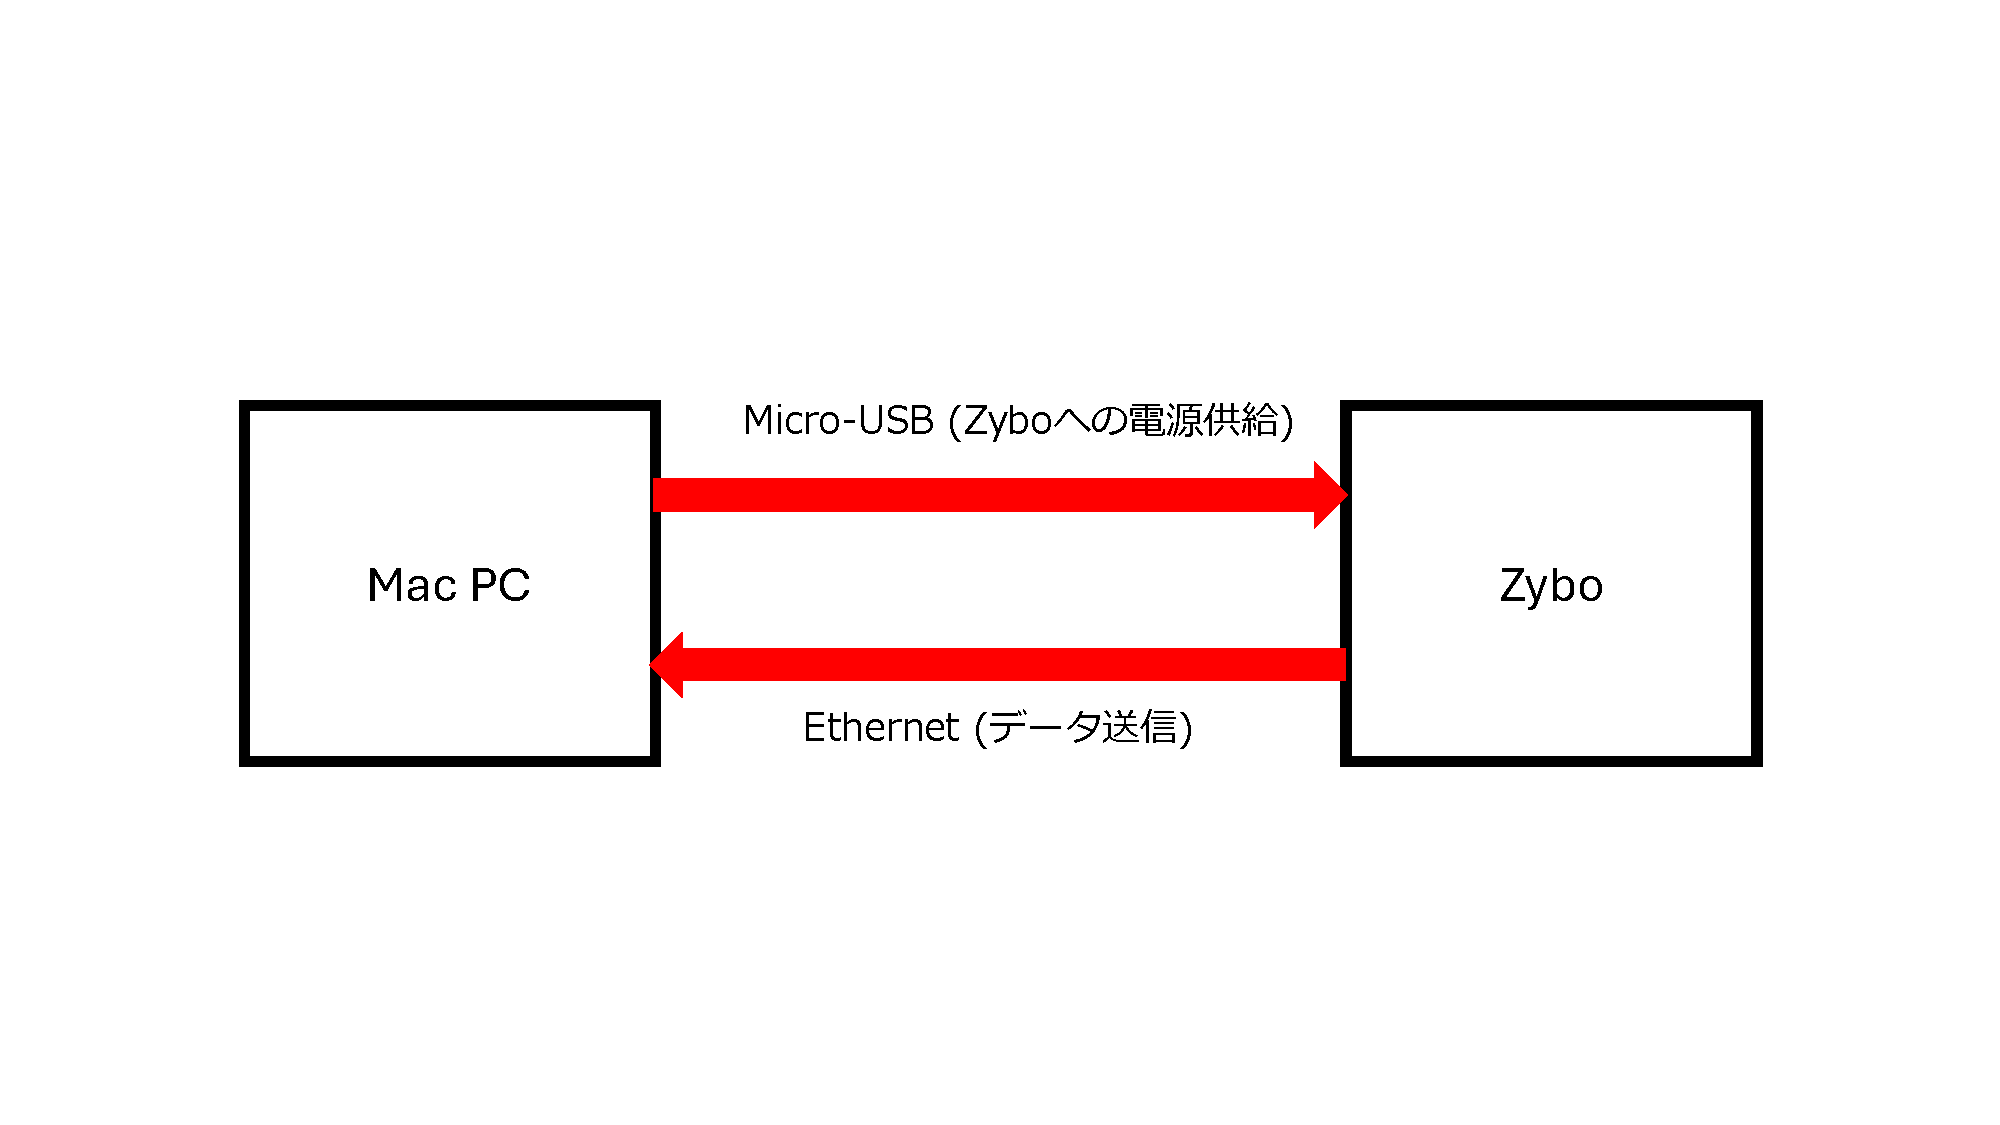
\includegraphics[keepaspectratio, scale=0.35]{4_elDAQ/figs/el_test2.pdf}
      \subcaption{セットアップの模式図}
    \end{minipage}
    %---- 図はここまで ----------------------
  \end{tabular}
  \caption{新システムでの動作確認}
  \label{el_test}
\end{figure}

動作確認を、図\ref{el_test}に示したセットアップで行なった。ロータリーエンコーダーとは接続せず、同期信号も送らない単純なものである。図\ref{el_test}の左図にあるように、Zyboの電源を入れPYNQが起動するとボード右側の``DONE''ランプが緑色に点灯する。自分のMac PCをデータ取得PCとして、Micro-USBでZyboへの電源供給を行い、データ通信はEthernetケーブルで行った。PC上でデータ読み出しのスクリプトを動かして、Zynqの挙動に問題がないかをチェックした。期待される挙動は
\begin{itemize}
  \item Zynqが正しく機能し、PC側でデータを読み出せる
  \item エンコーダーデータは0として取得されている
  \item タイムスタンプは時間とともに加算されている
\end{itemize}
の3点である。データの通信が始まるとZyboのEthernetコネクタ付近のランプが点滅し、PC側でのデータ読み出しが正常に動くことを確認した。PCに保存したデータファイルをチェックし、期待されるデータを取得できていることも確認した。取得したエンコーダーデータとタイムスタンプデータのプロットを図\ref{eldata_check}に示す。プロットの横軸はデータのサンプリングナンバー(1kSPS)を表す。

\begin{figure}[h]
  \begin{tabular}{cc}
    %---- 最初の図 ---------------------------
    \begin{minipage}[t]{0.45\hsize}
      \centering
      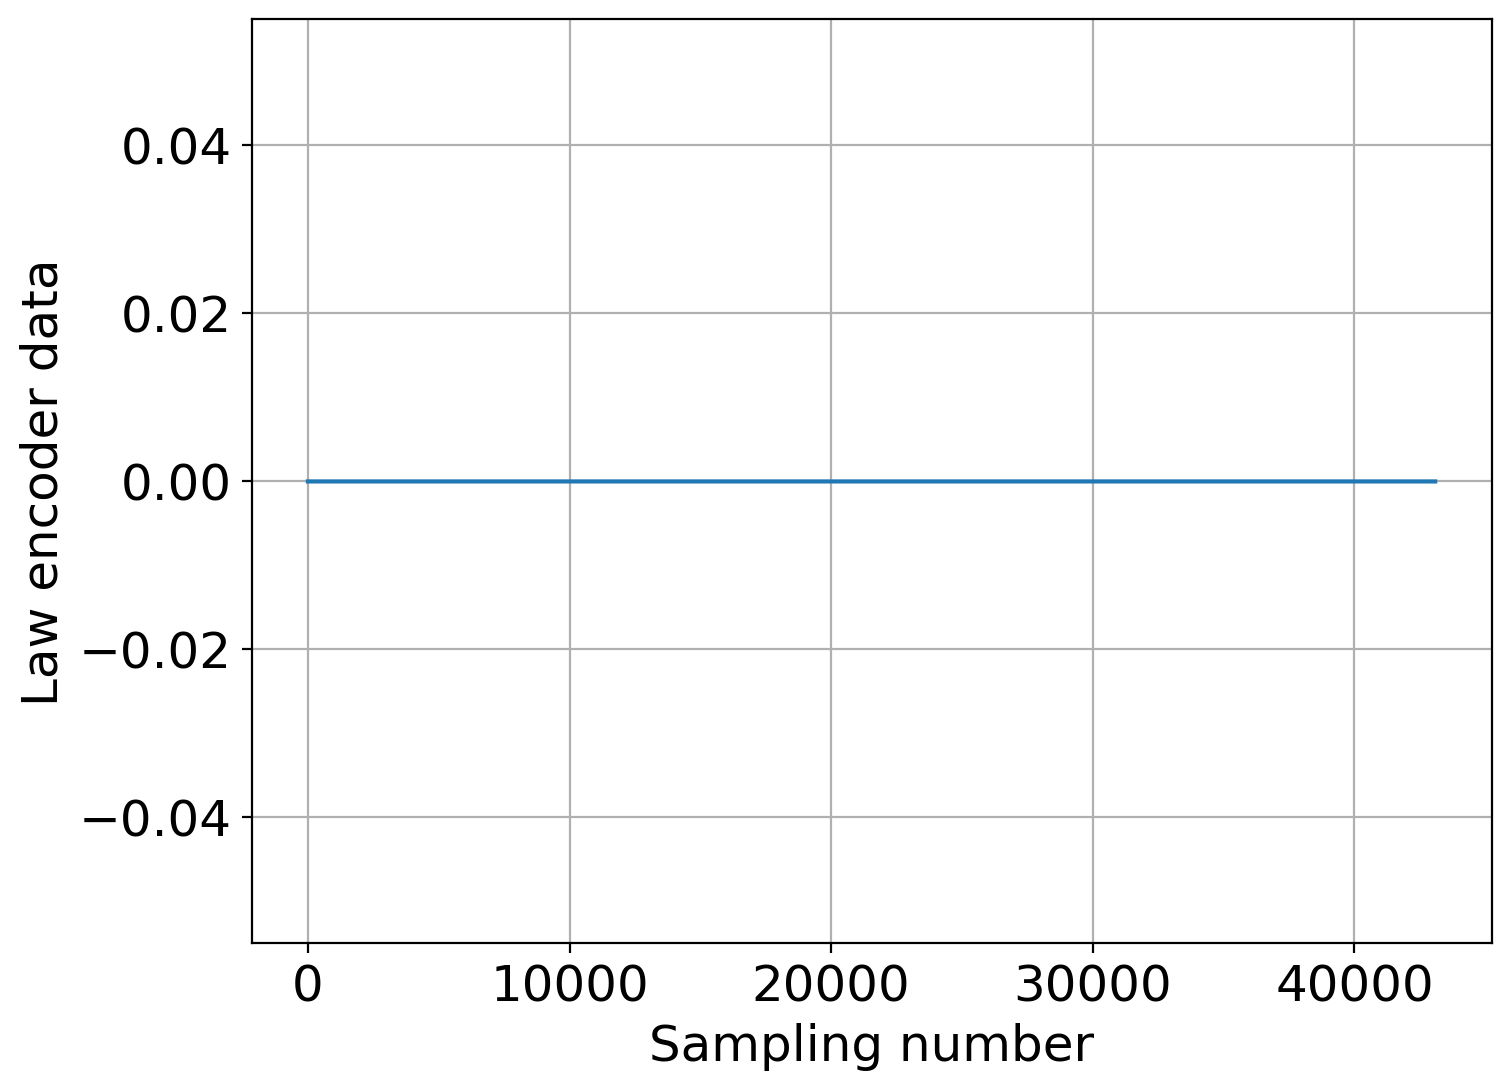
\includegraphics[keepaspectratio, scale=0.35]{4_elDAQ/figs/enc_data_test.png}
      \subcaption{エンコーダーデータ}
    \end{minipage}
    %---- 2番目の図 --------------------------
    \begin{minipage}[t]{0.45\hsize}
      \centering
      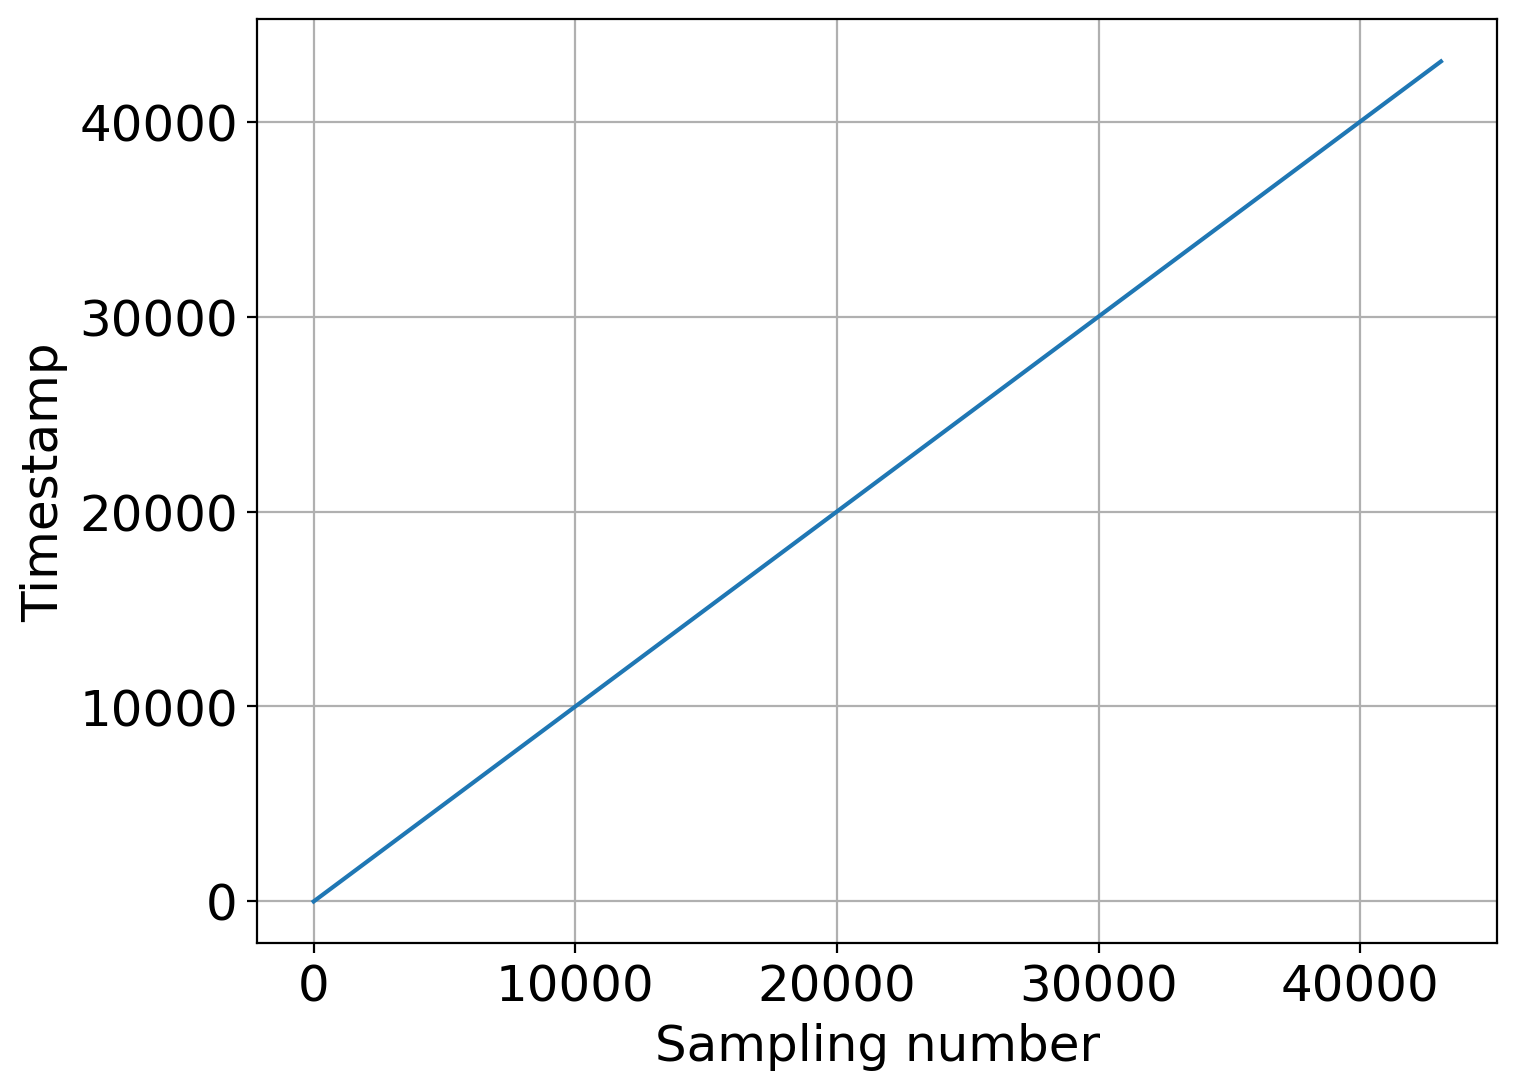
\includegraphics[keepaspectratio, scale=0.35]{4_elDAQ/figs/timestamp.png}
      \subcaption{タイムスタンプ}
    \end{minipage}
    %---- 図はここまで ----------------------
  \end{tabular}
  \caption{動作確認で取得したデータ}
  \label{eldata_check}
\end{figure}

以上の結果から新システムの挙動が問題ないと判断し、次に実際の望遠鏡にインストールした。インストールはSDカードを新システムのものに交換するだけで完了し、PYNQの起動を確認した。

\begin{figure}[h]
  \begin{tabular}{cc}
    %---- 最初の図 ---------------------------
    \begin{minipage}[t]{0.45\hsize}
      \centering
      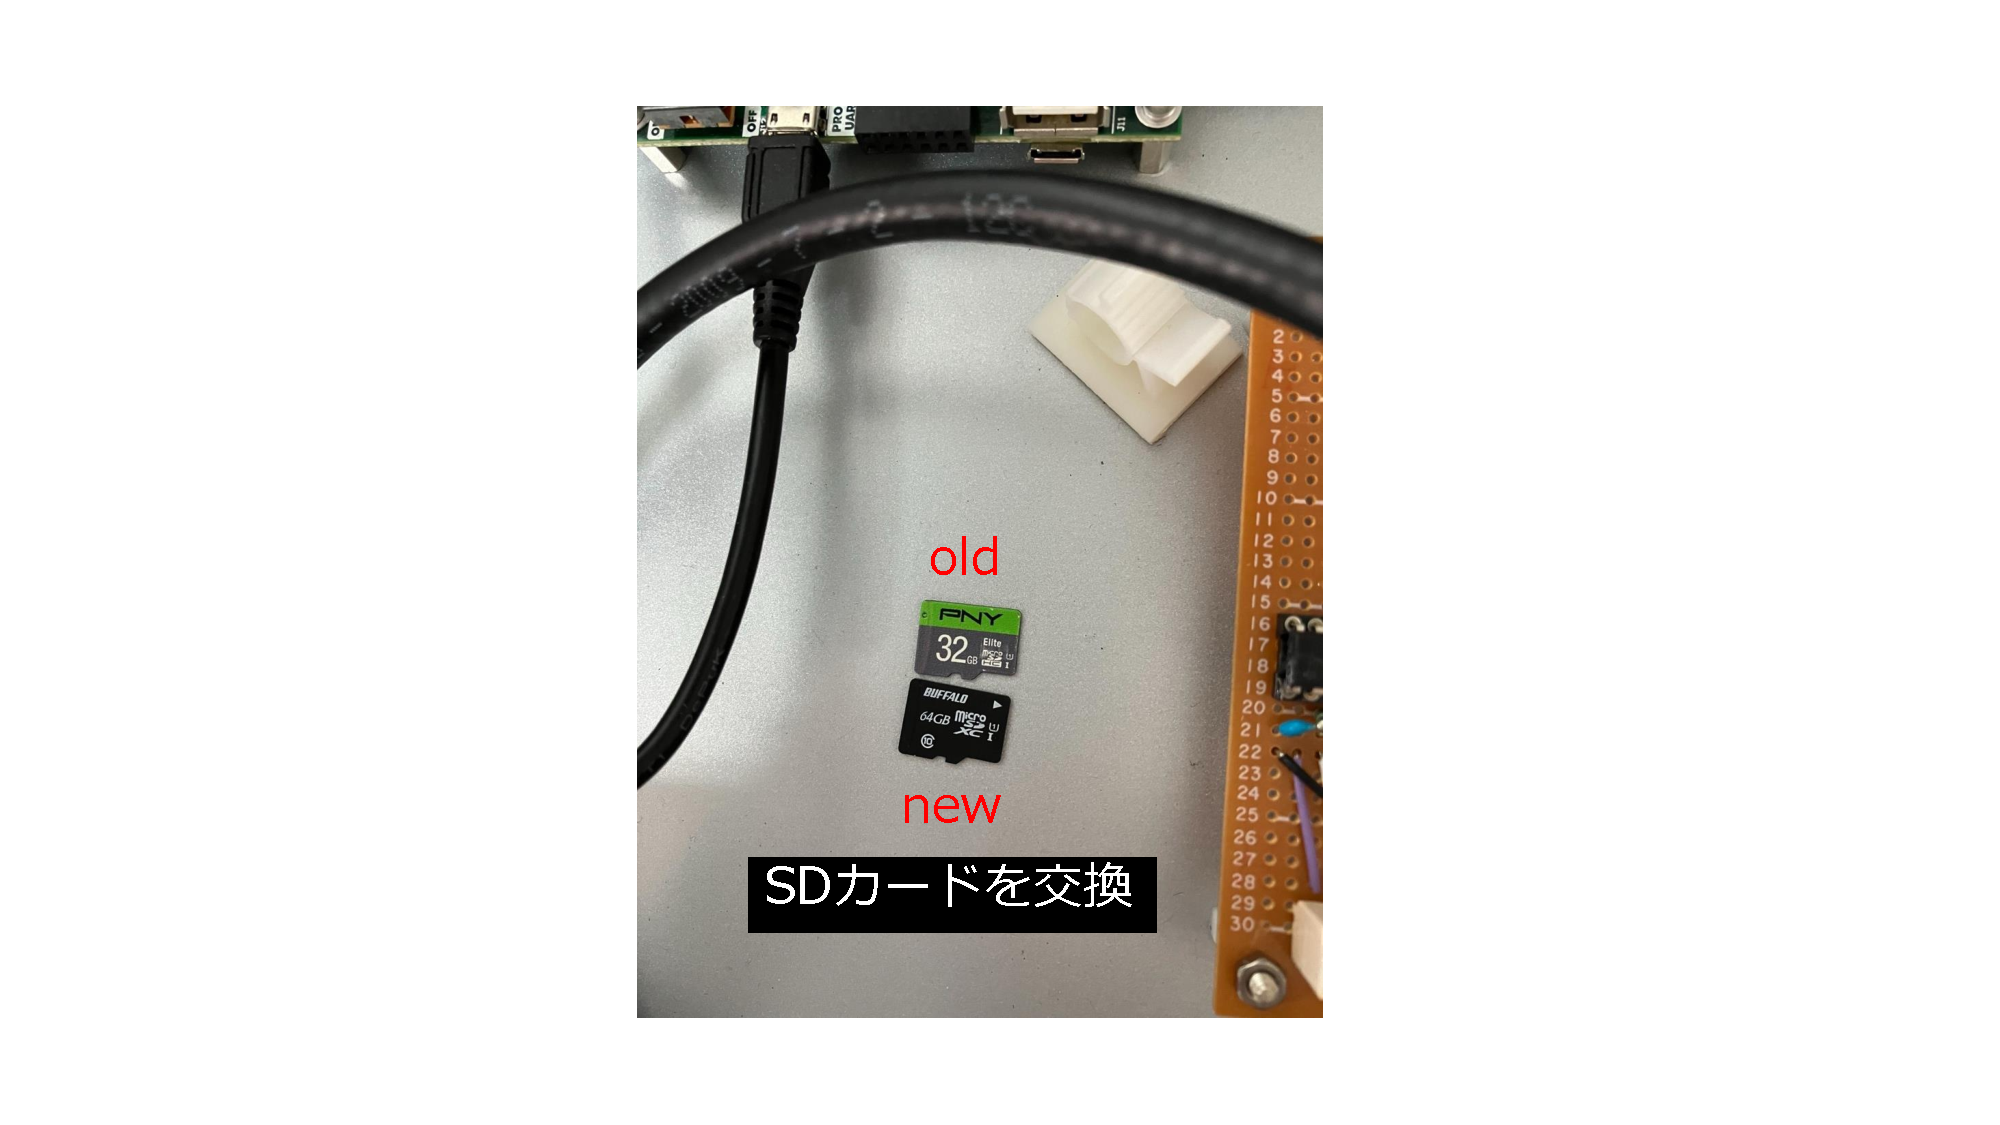
\includegraphics[keepaspectratio, scale=0.35]{4_elDAQ/figs/sd_exchange.pdf}
      \subcaption{SDカードの交換}
    \end{minipage}
    %---- 2番目の図 --------------------------
    \begin{minipage}[t]{0.45\hsize}
      \centering
      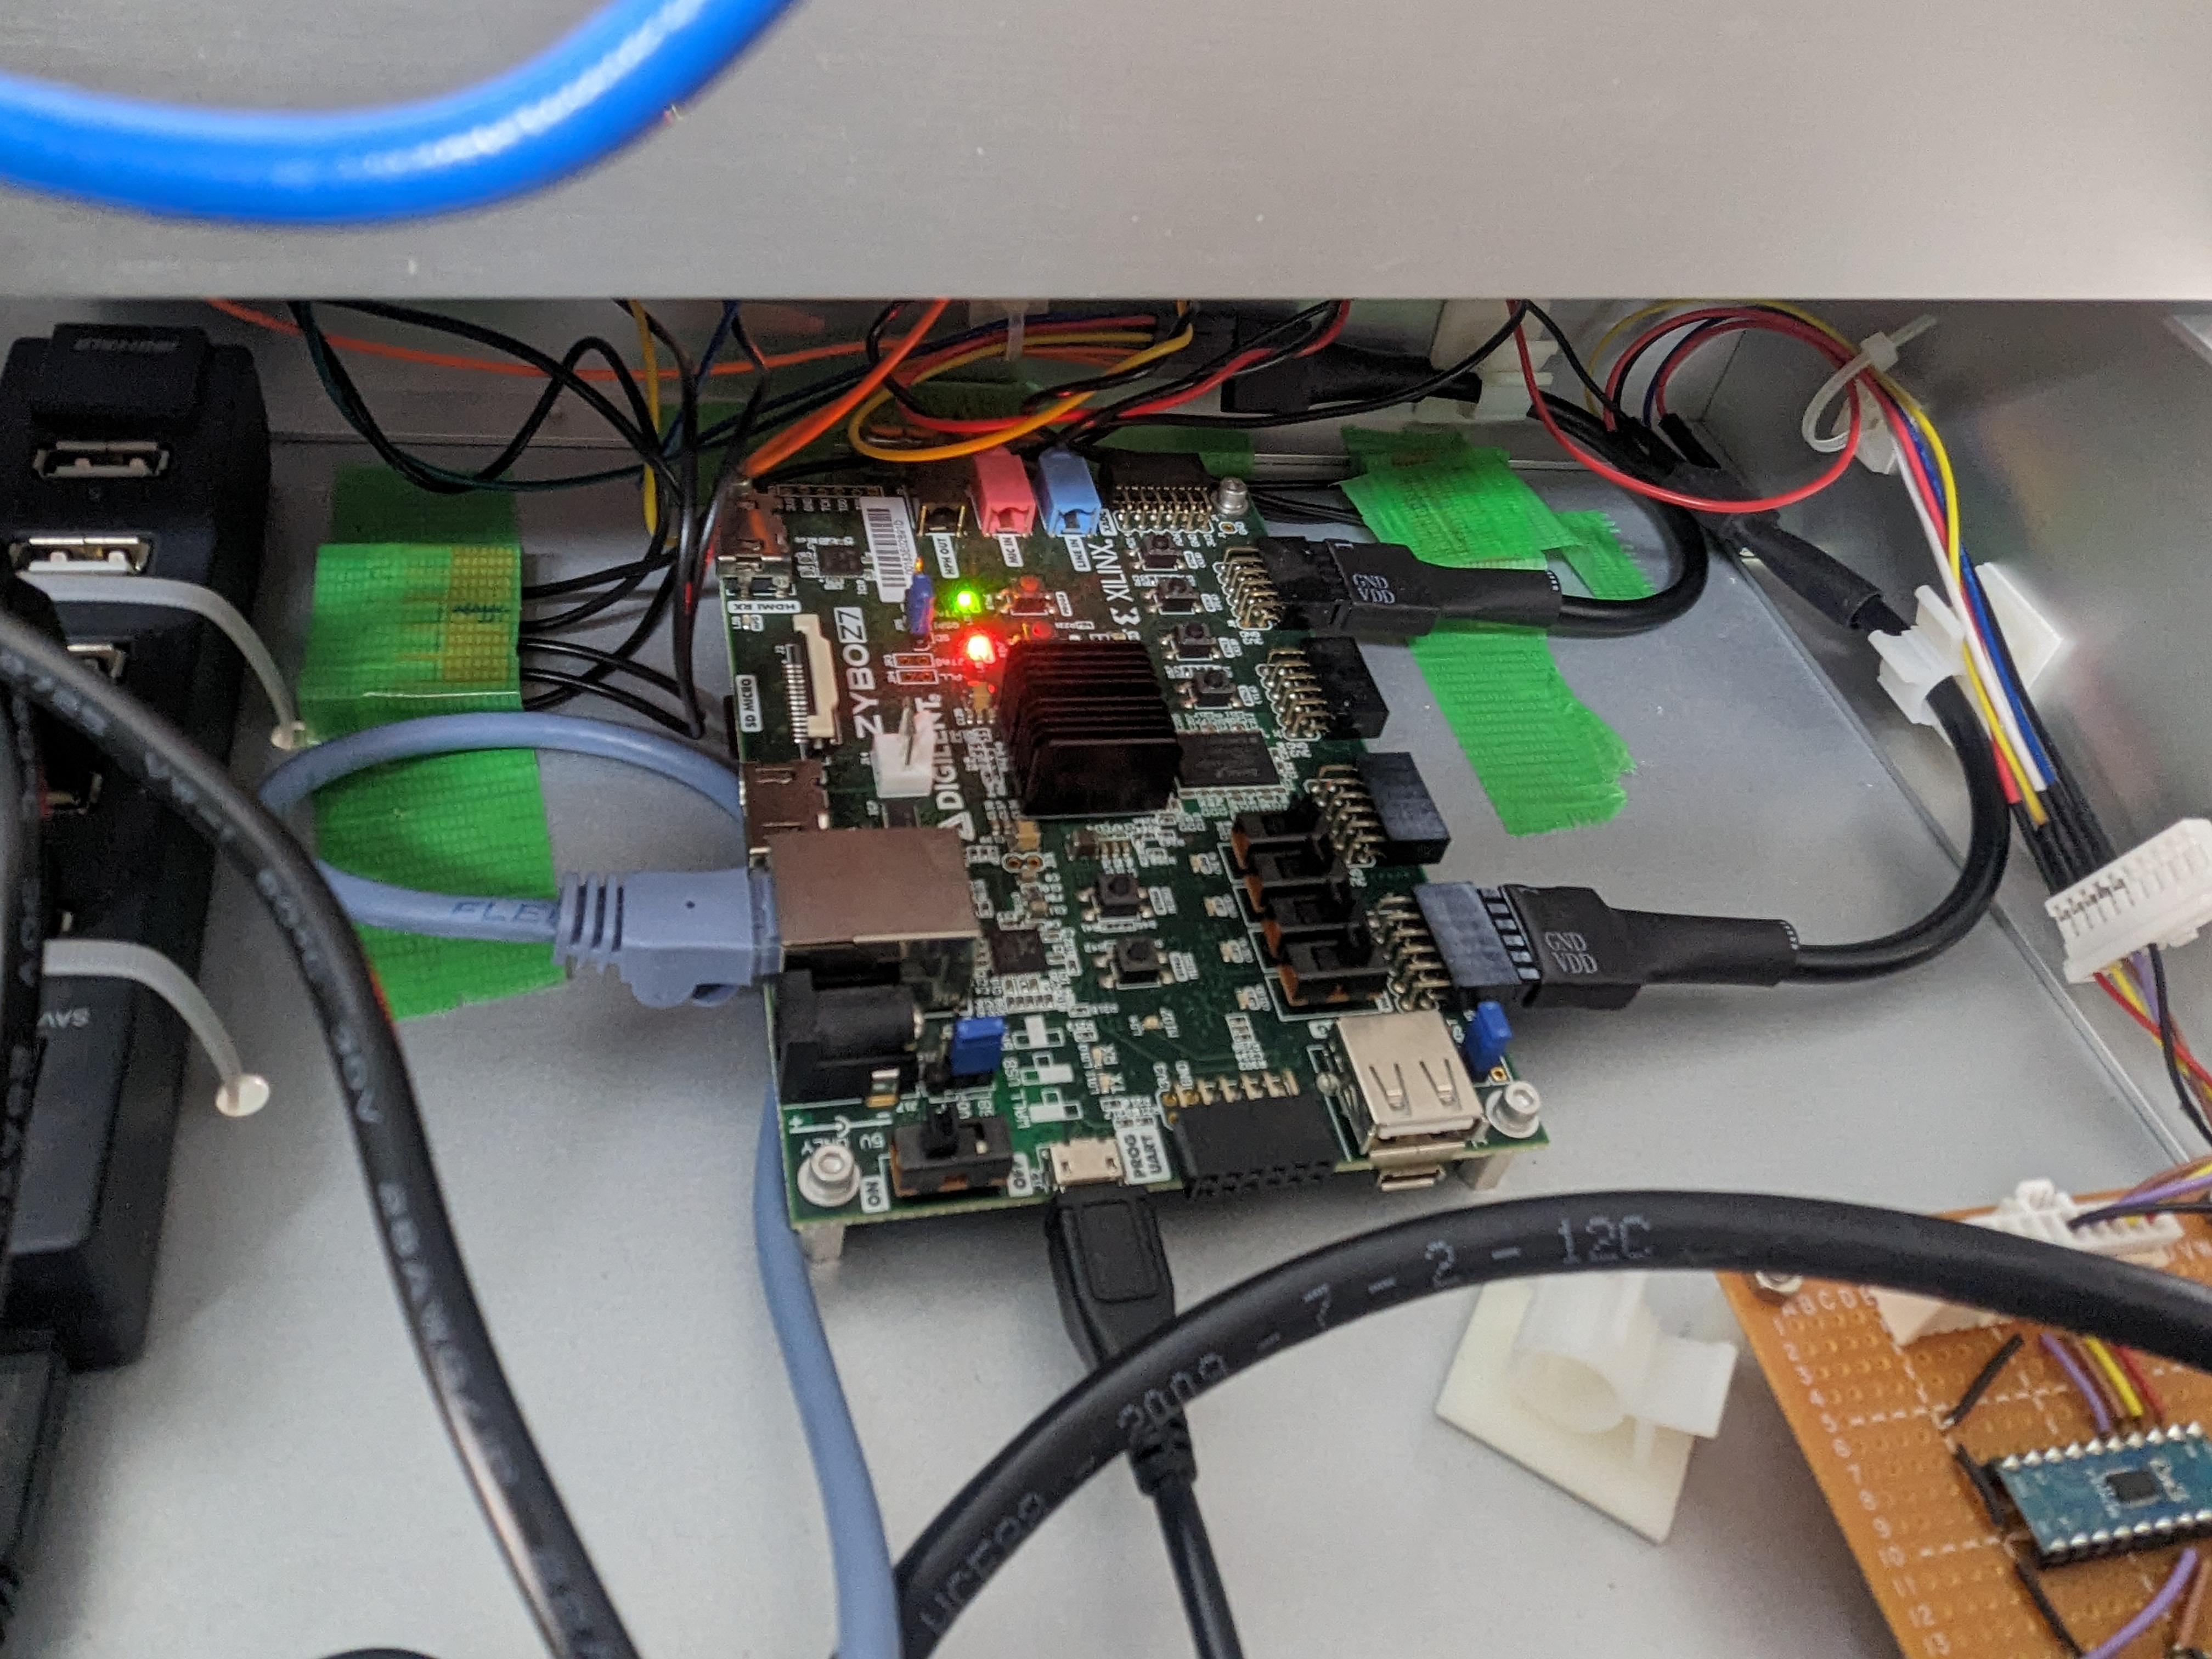
\includegraphics[keepaspectratio, scale=0.048]{4_elDAQ/figs/pynq_start.jpg}
      \subcaption{PYNQの起動}
    \end{minipage}
    %---- 図はここまで ----------------------
  \end{tabular}
  \caption{新システムのインストール}
  \label{el_install}
\end{figure}

\subsection{同期信号取得の確認}
インストール後に実際の望遠鏡システムでデータを読み出せるかの動作確認を行なった。まず、方位角DAQからの同期信号を正しく取得して仰角データとして保存できているのかを確認した。結果を図\ref{sync_id}に示す。同期信号は1秒に1回出力されるので、仰角データでは同期信号の番号(図では``Sync\_id''と記す)が1秒で1ずつ増加する形で見えるはずであり、その結果を確認することができた。

\begin{figure}[htbp]
  \centering
  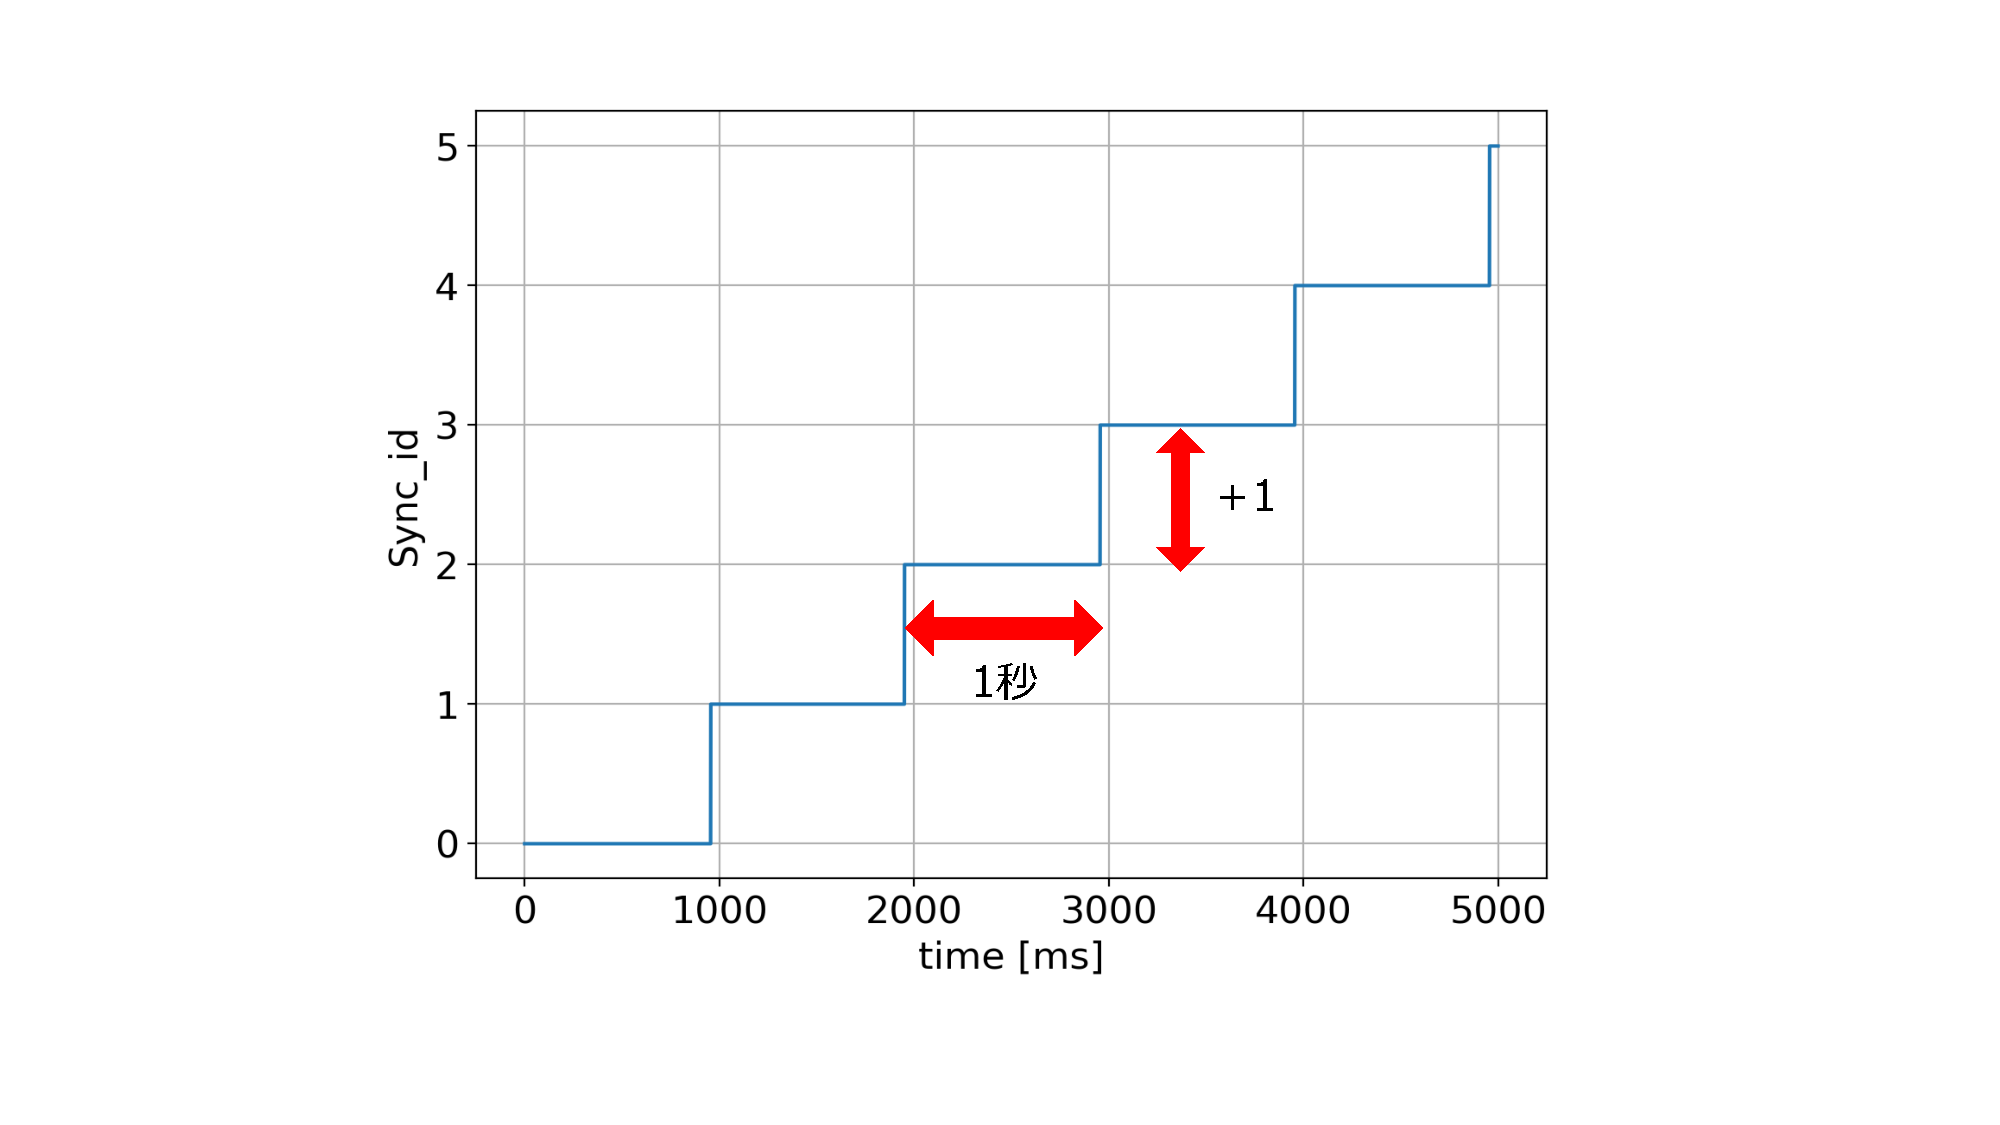
\includegraphics[width=0.8\columnwidth]{4_elDAQ/figs/sync_id.pdf}
  \caption{仰角データからみた同期信号。方位角DAQからの同期信号を取得するごとに``Sync\_id''が1ずつ加算される。}
  \label{sync_id}
\end{figure}

\subsection{同期信号の分配と仰角データ取得の確認}
次に、取得した同期信号をMKID DAQに分配できていることと仰角データを正しく読み出せているかを確認した。一度失ったエンコーダーの原点情報を再度取得するためにも、望遠鏡の仰角を$90^{\circ}$と$70^{\circ}$の間で何度か動かして、さらに並行してMKIDのデータも取得した。それらのデータを使って確認を行なった。確認の手順は以下である。
\begin{enumerate}
  \item テスト用として取ったMKIDデータを読み出す
  \item 正しく動作していればMKIDデータに同期した時間情報と仰角データを取得できる
  \item その仰角データが正しい値を読み出せているかを確認
\end{enumerate}

結果を図\ref{elevation_data}に示す。MKIDデータから同期情報を取得でき、読み出した仰角データが$90^{\circ}$と$70^{\circ}$の間で正しく動いていることも確認した。

\begin{figure}[htbp]
  \centering
  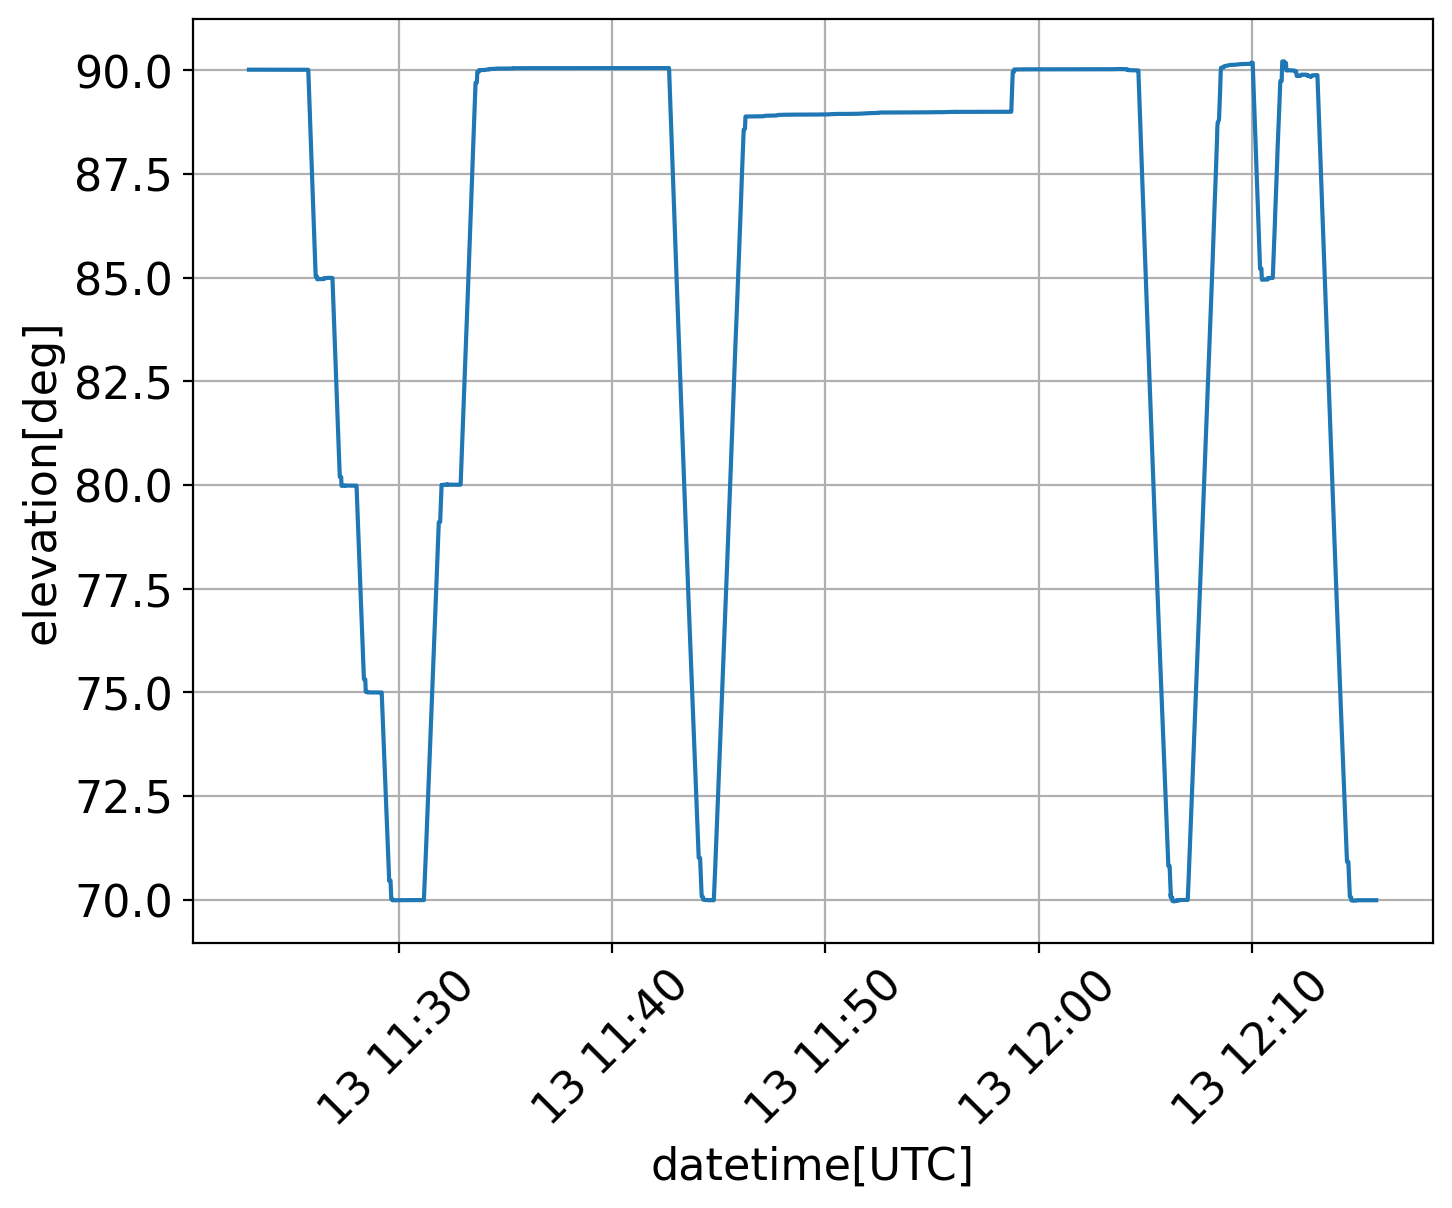
\includegraphics[width=0.8\columnwidth]{4_elDAQ/figs/elevation_data.png}
  \caption{読み出した仰角データ。横軸(2024/3/13のUTC時間)の時間情報が実際の作業時間とリンクしており、MKIDデータで同期信号が正しく取得できていることを反映している。}
  \label{elevation_data}
\end{figure}

以上から新システムが実際の望遠鏡で問題なく動作することを確認した。その後、動作が安定して長期間行われるかをチェックした。

\section{メンテナンスと安定運用}

\subsection{動作の不安定性}
インストール後、動作の安定性に問題があり、データ取得が途切れることが何度か発生した。途切れる原因はZyboの電源が一時的に落ちることによるものであった。インストール時の動作確認で問題がなかったことから、Zynq内でのデータ処理と通信自体に問題がある可能性はないと考えた。他に原因となりうるものは
\begin{itemize}
  \item OSが搭載されたことでZyboの消費電力が上がり、一時的に電源供給量が足りなくなる
  \item Zynqでの消費電力も上がり、Zynqの温度が許容値よりも高くなってしまう
  \item そもそもZyboのボード自体がどこかで劣化している
\end{itemize}
が挙げられる。3つ目に関しては、経年劣化や落雷による停電時にダメージを受けたことなどが考えられるが、リモートからボード自体の性能を評価することが難しいため、まずは1つ目と2つ目の原因について調査した。

\subsection{電源供給方法の見直し}
Zyboへの電源供給は図\ref{el_install}の右図にあるように、Micro-USB端子から行なっていた。Zyboへの電源供給方法は他にジャック端子から(図\ref{power_ supply})がある。

\begin{figure}[htbp]
  \centering
  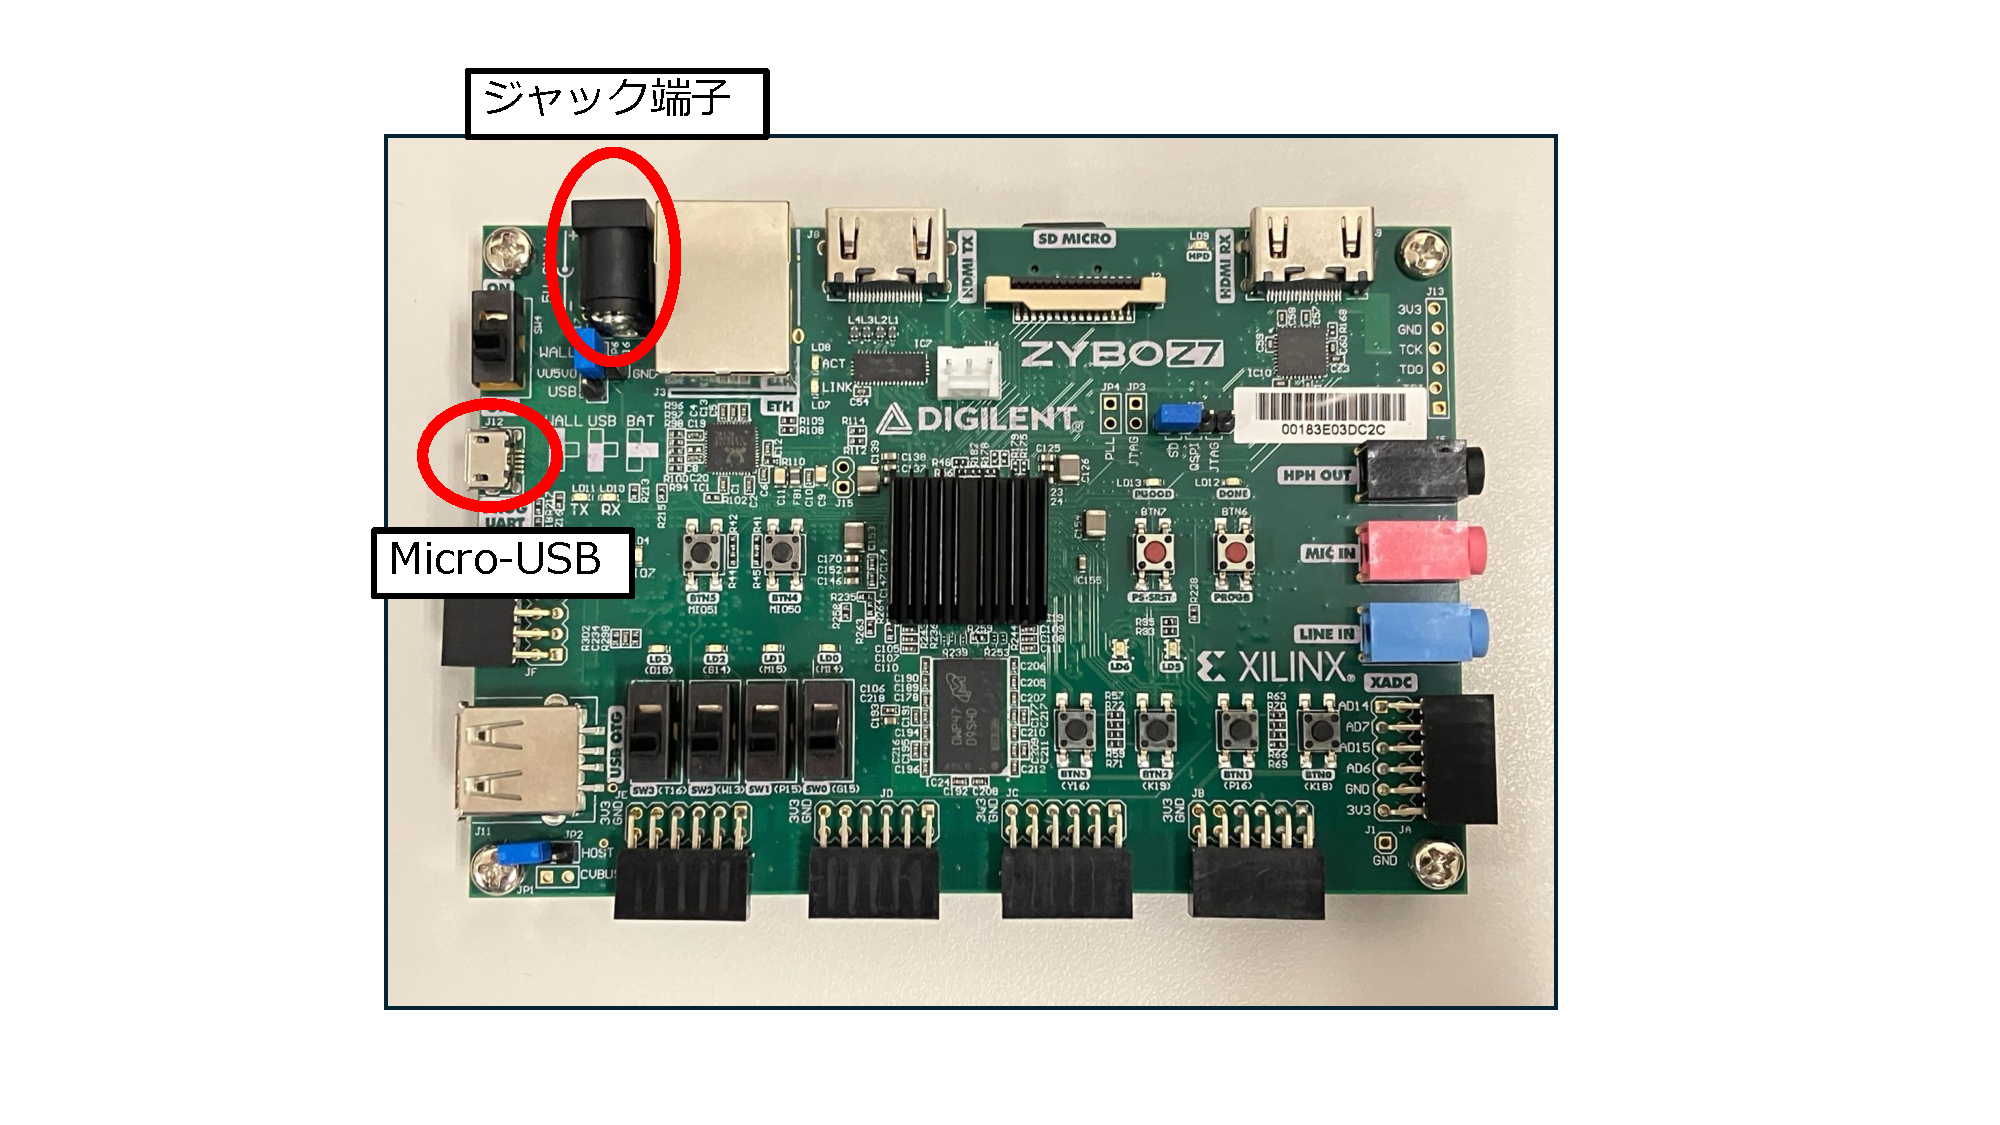
\includegraphics[width=0.5\columnwidth]{4_elDAQ/figs/connector_zybo2.pdf}
  \caption{Zyboへの電源供給方法。Micro-USBからとジャック端子からの2通りがある。}
  \label{power_supply}
\end{figure}

この2種類の供給方法について比較すると表\ref{power_spec}のようになる。ジャック端子については標準的なACアダプタの規格を参照する。

\begin{table}[htbp]
  \centering
  \caption{各電源供給方法での定格値}
  \vspace{3mm}
  \begin{tabular}{cccc} \hline
    供給方法 & 定格電圧 & 定格電流 & 接続の安定性  \\ \hline
    Micro-USB & 5V & 最大0.5A & やや不安定\\
    ジャック端子 & 5V & 最大4A &  安定\\ \hline
  \end{tabular}
  \label{power_spec}
\end{table}

これより、供給できる電力量や接続の安定性に関してジャック端子の方が優れていることが分かる。特に定格電流の値が大きく異なっており、従来のシステムではMicro-USBからの給電で間に合っていたが、OSが搭載されたことで給電が足りなくなった可能性が考えられる。スペックシート\cite{power_ref}でもジャック端子による電源供給が推奨されている(参考として、電力を大量に消費する処理をZynqに搭載した場合は12.5W以上の出力が必要)。そのため、Zyboへの電源供給方法をジャック端子に変更して十分な電力を供給することで動作の安定性を図るのが良いと考えた。変更するにあたって新システムを稼働した際のZyboの安定性を給電条件を変えてテストした。行なったテストの様子を図\ref{power_test}に、給電条件と結果を表\ref{power_result}に示す。

\begin{figure}[htbp]
  \begin{tabular}{cc}
    \begin{minipage}[t]{0.45\hsize}
      \centering
      \includegraphics[width=0.5\columnwidth]{4_elDAQ/figs/test_usb.jpg}
      \subcaption{テスト1}
    \end{minipage} &
    \begin{minipage}[t]{0.45\hsize}
      \centering
      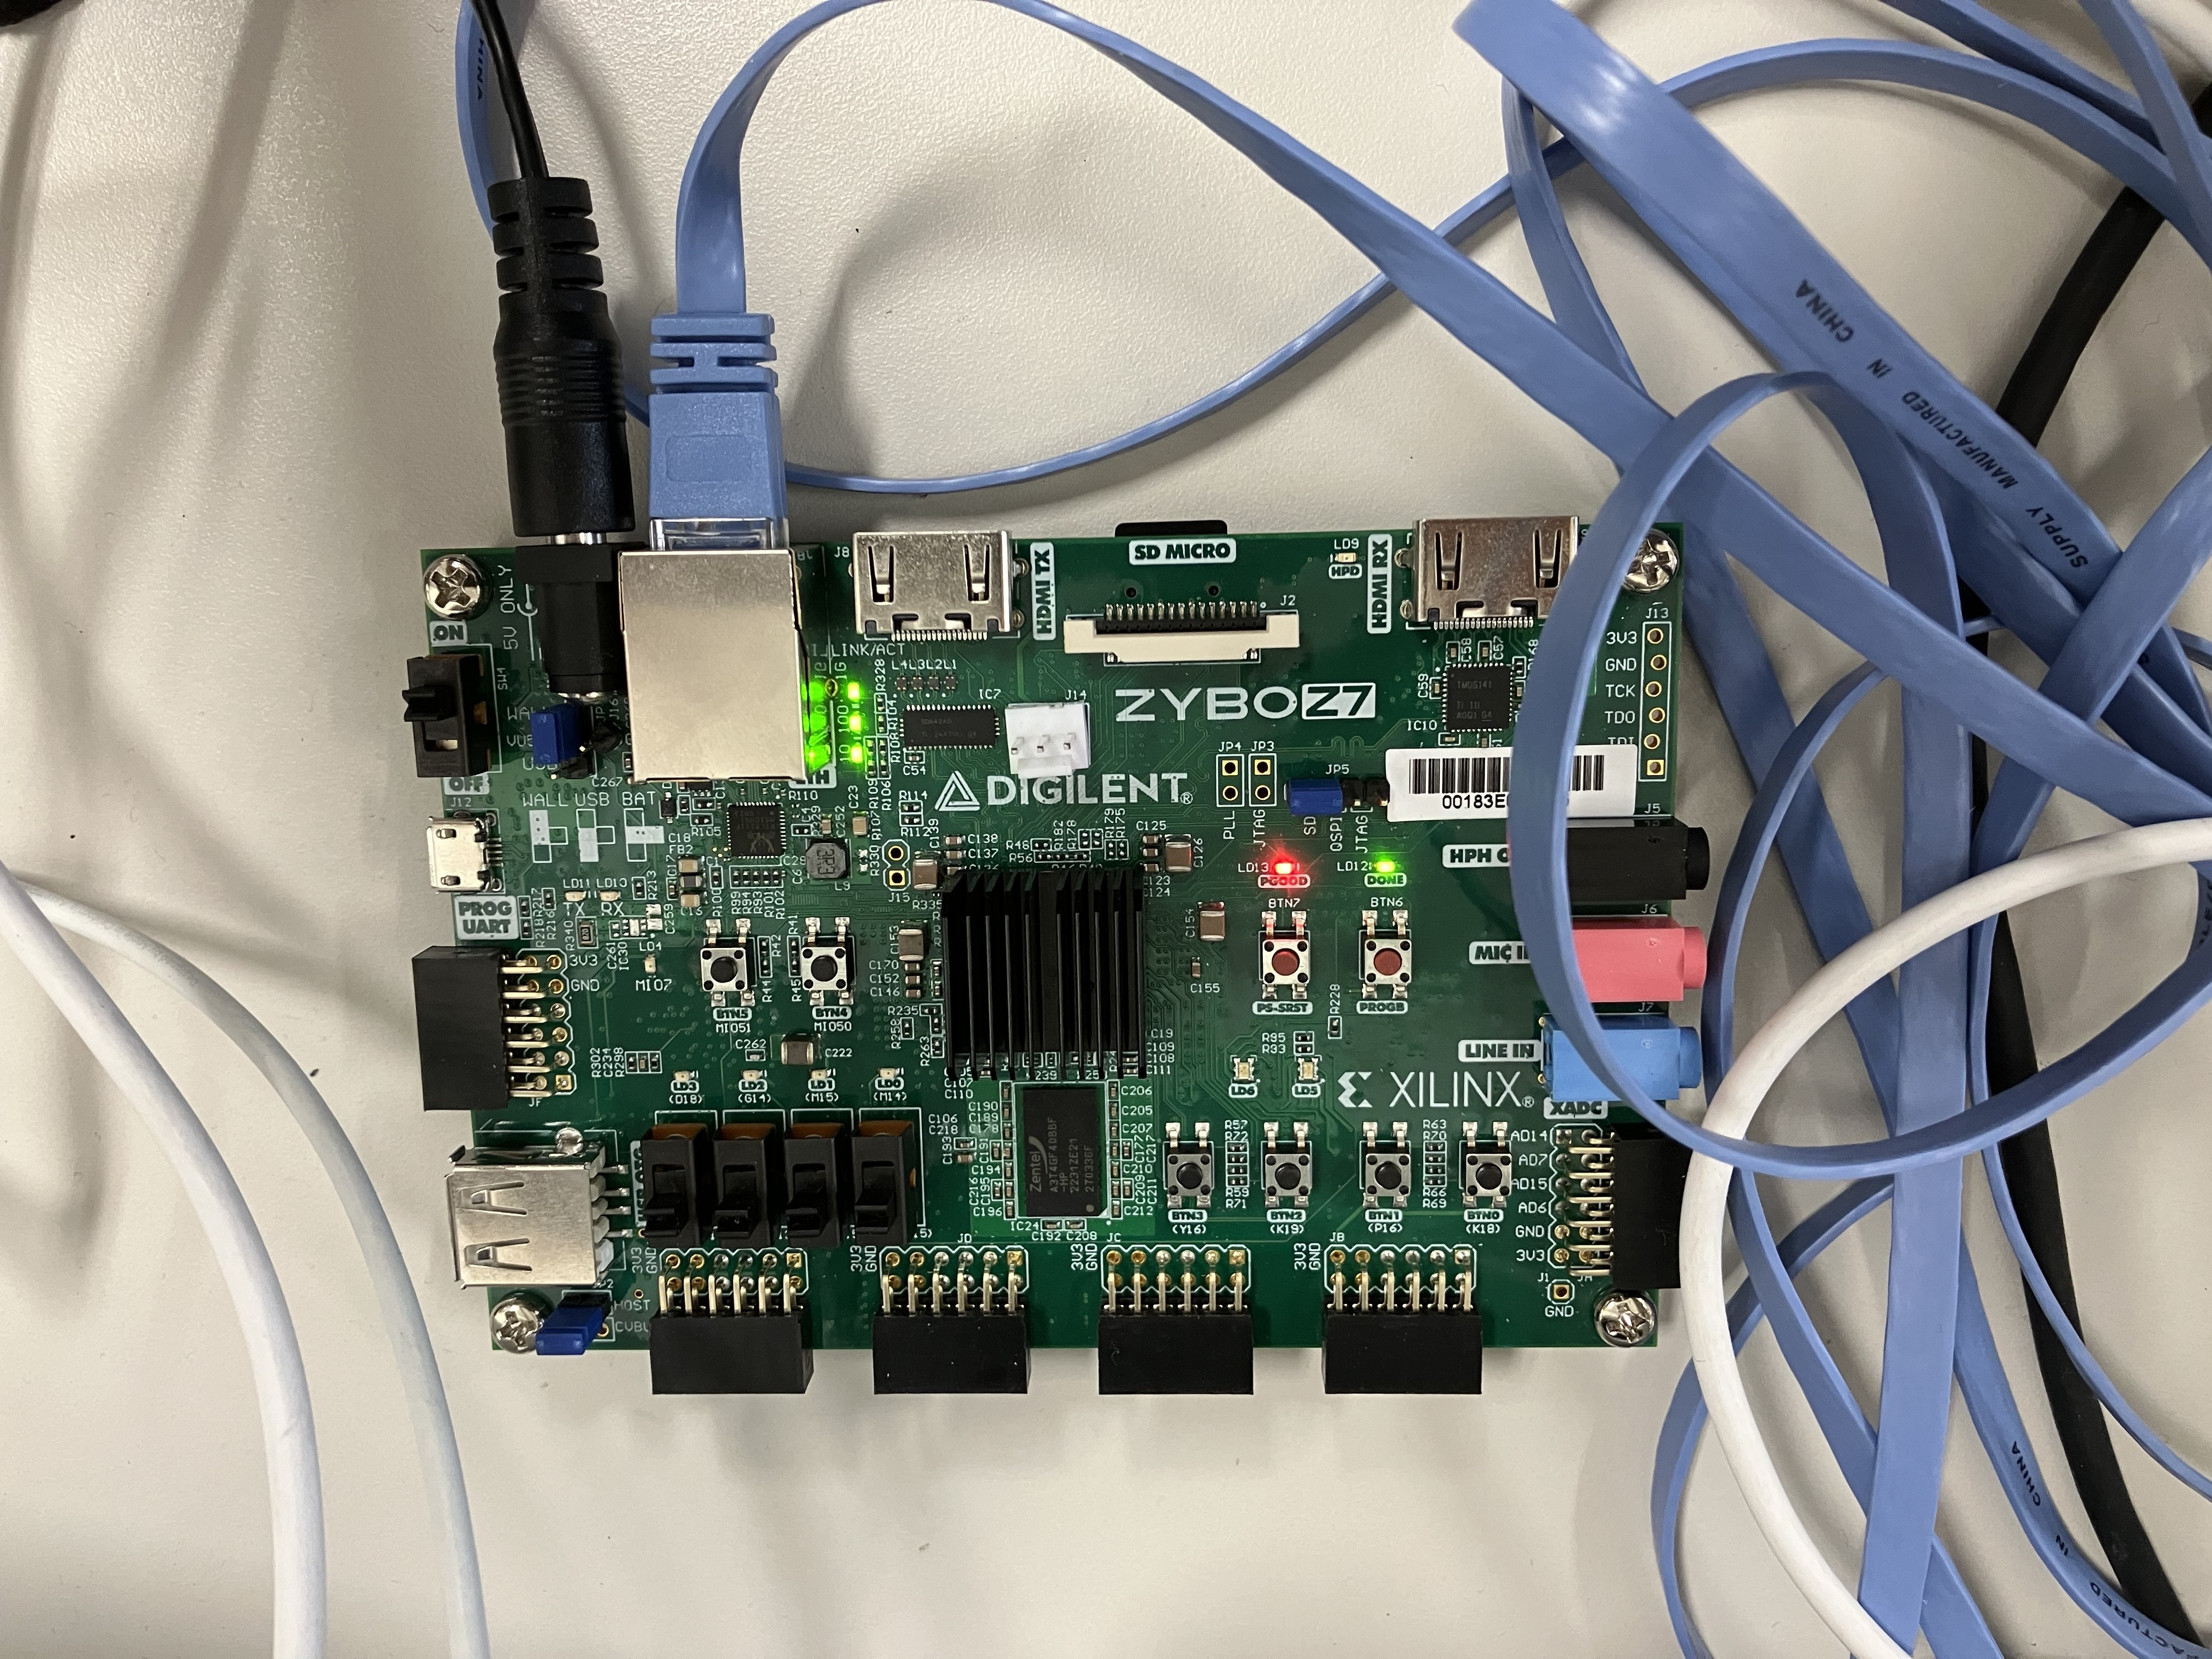
\includegraphics[width=0.5\columnwidth]{4_elDAQ/figs/test_jack.jpg}
      \subcaption{テスト2}
    \end{minipage} \\

    \begin{minipage}[t]{0.45\hsize}
      \centering
      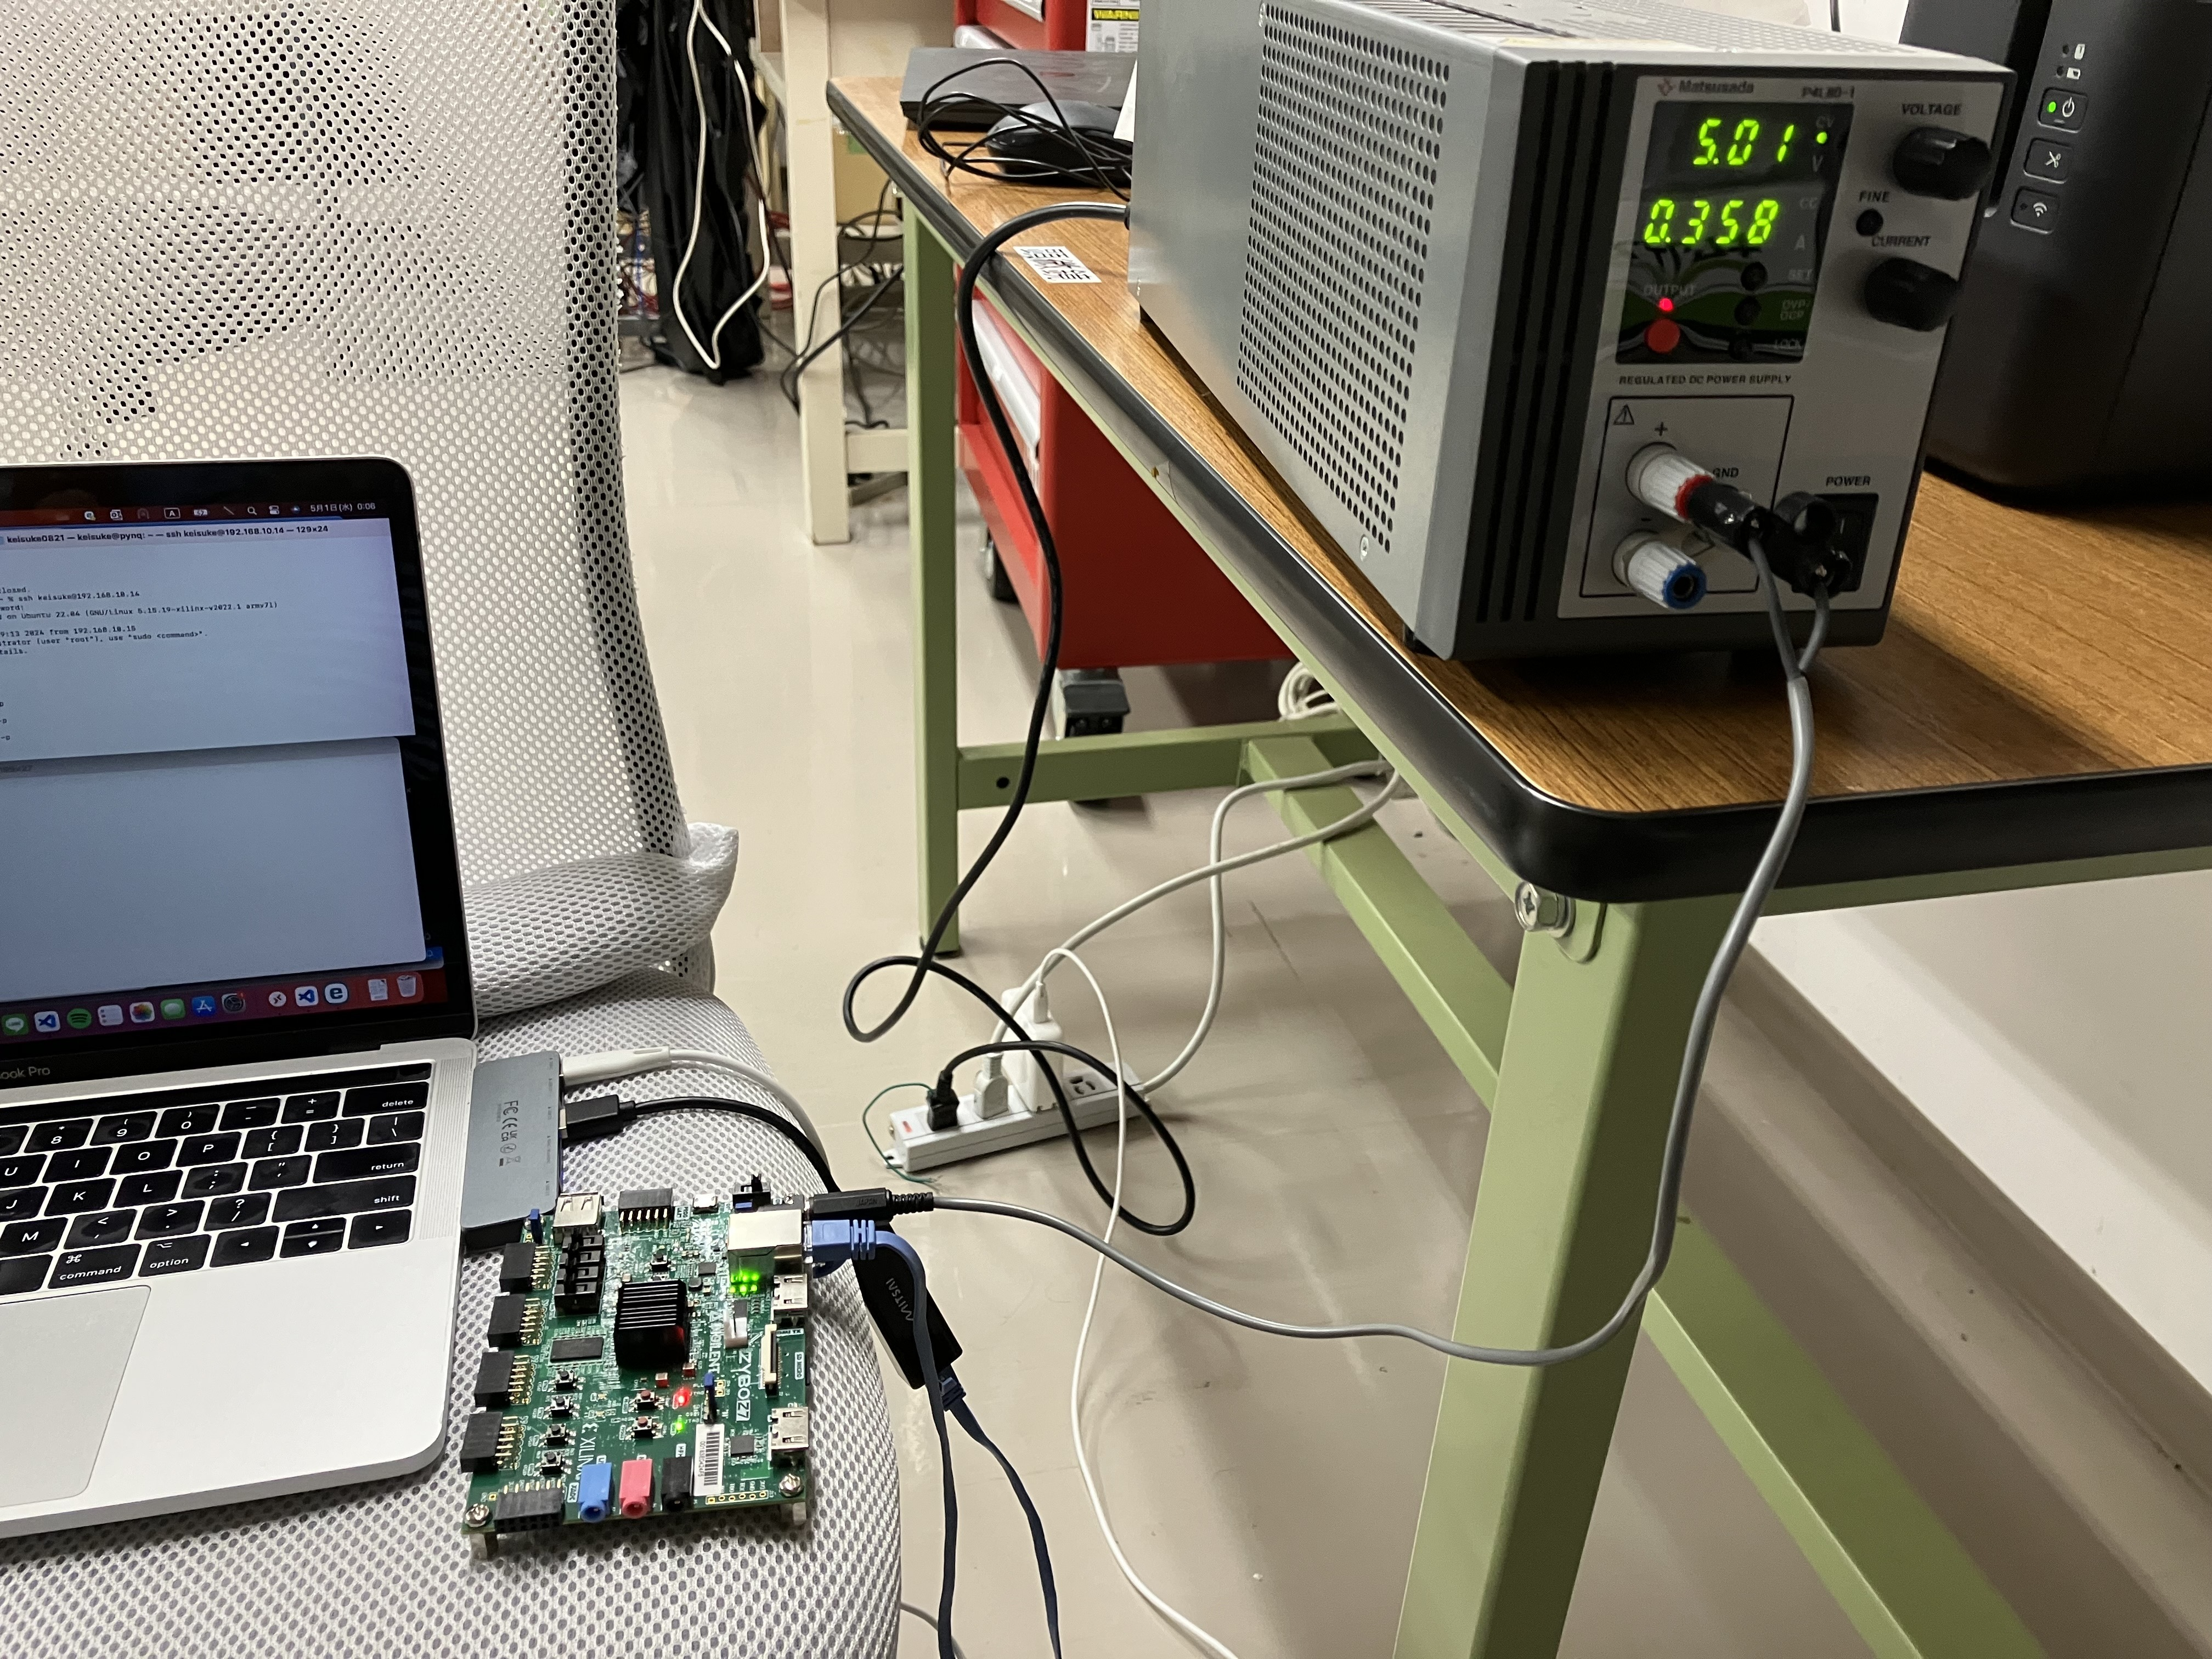
\includegraphics[width=0.5\columnwidth]{4_elDAQ/figs/test_50.jpg}
      \subcaption{テスト3}
    \end{minipage} &
    \begin{minipage}[t]{0.45\hsize}
      \centering
      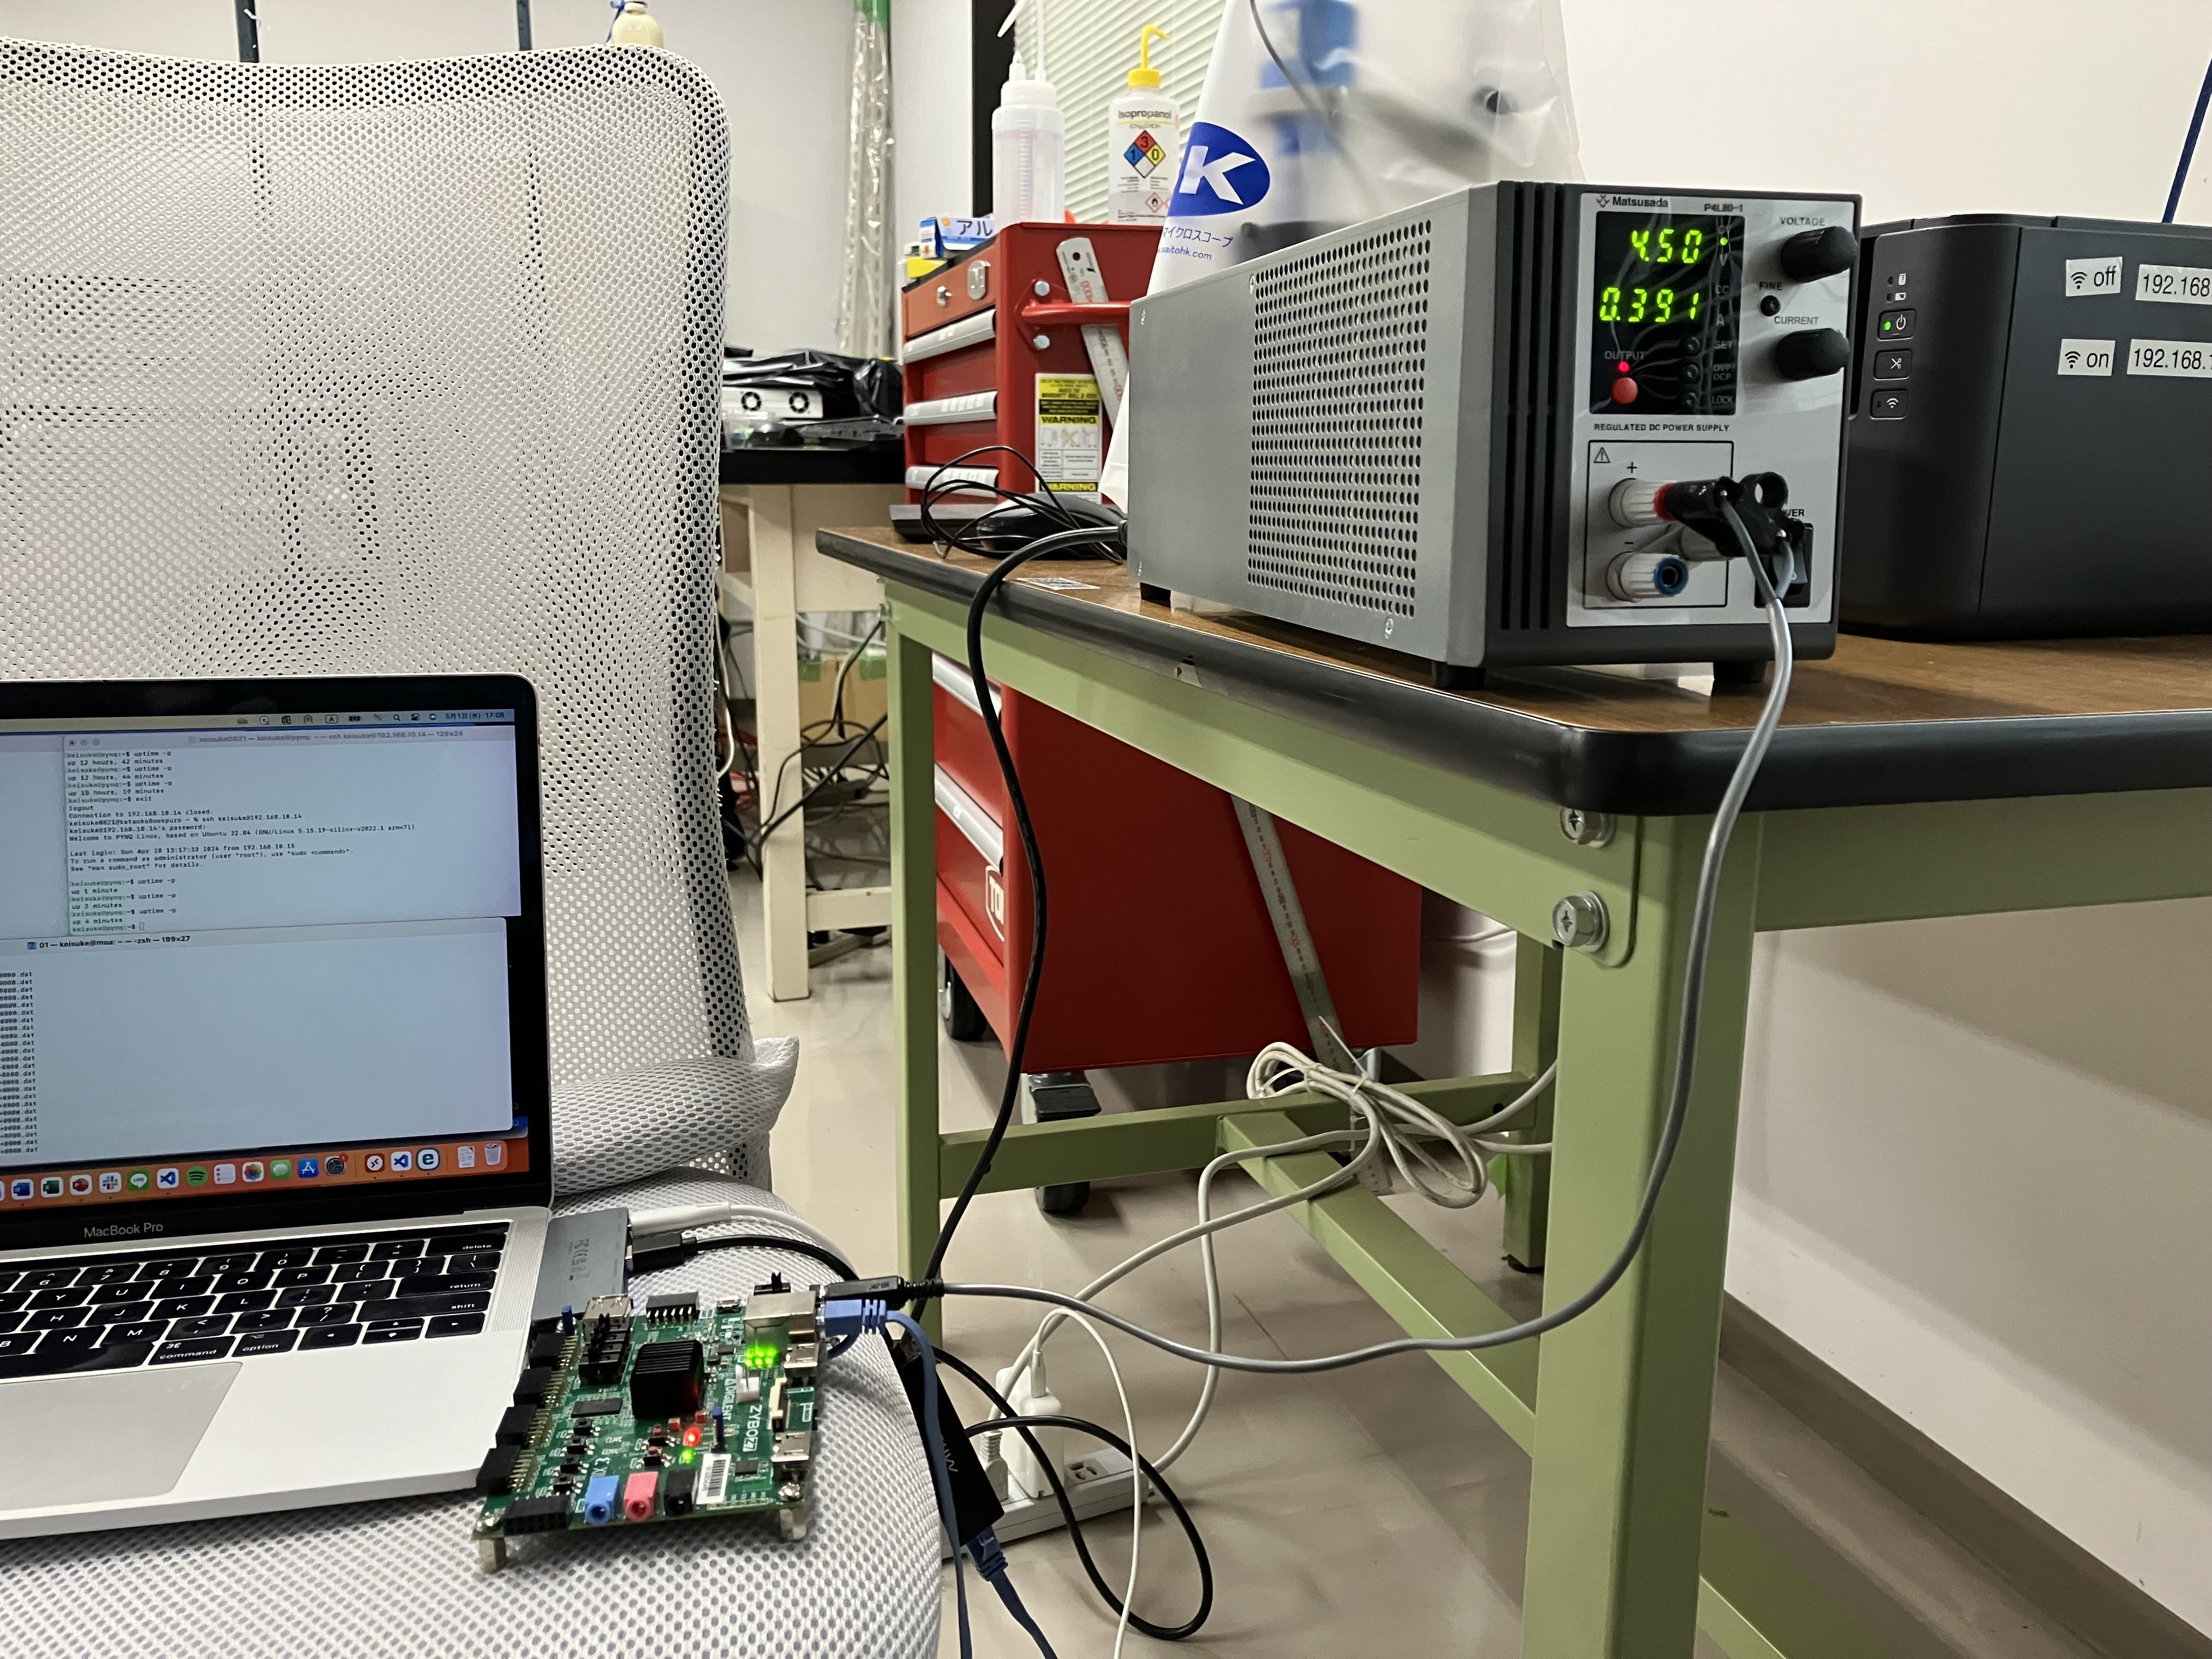
\includegraphics[width=0.5\columnwidth]{4_elDAQ/figs/test_45.jpg}
      \subcaption{テスト4}
    \end{minipage}
  \end{tabular}
   \caption{Zyboの安定稼働テスト}
   \label{power_test}
\end{figure}

\begin{table}[htbp]
  \centering
  \caption{安定稼働テストの給電条件と結果}
  \vspace{3mm}
  \begin{tabular}{ccc} \hline
     & 給電条件 & 動作の結果  \\ \hline
    テスト1 & 従来と同じUSB & 安定 \\
    テスト2 & ジャック端子(5V、4AのACアダプタ) & 安定 \\ \hline
    テスト3 & 直流電源(定電圧モード 5.0V) & 安定 \\
    テスト4 & 直流電源(定電圧モード 4.5V) & 不安定(DAQ開始後数時間でZyboの電源が落ちる)  \hline
  \end{tabular}
  \label{power_result}
\end{table}

\subsection{Zynq温度のモニター}
